\documentclass[a4paper,13pt]{report}
\usepackage[utf8]{inputenc}
\usepackage[final]{microtype}
\usepackage{amsmath}
\usepackage{amsfonts}
\usepackage{amssymb}
\usepackage{graphicx}
\usepackage{xspace}
\usepackage[font=small]{caption}
\usepackage{booktabs}
\usepackage[unicode]{hyperref}
\usepackage[left=3cm,right=2cm,top=2.5cm,bottom=3cm]{geometry}
\usepackage{titlesec}
\usepackage{scrextend}
\usepackage{enumitem}
\usepackage{url}
\PassOptionsToPackage{table}{xcolor}
\usepackage{tikz}
\usepackage{float}
\usepackage{afterpage}
\usepackage{multirow}
\usepackage{sectsty}
\usepackage{tocloft,calc}
\usepackage{listings}
\usepackage{makecell}
\usepackage{array}
\usepackage[sort&compress]{natbib}
\usetikzlibrary{calc,positioning,backgrounds,fit,shapes.geometric,arrows.meta}
\usepackage{algorithm}
\usepackage{algorithmic}
\usepackage{subcaption}
\usepackage[flushleft]{threeparttable}
\usepackage{needspace}
\usepackage{perpage}
\MakePerPage{footnote}

\def\changemargin#1#2{\list{}{\rightmargin#2\leftmargin#1}\item[]}
\let\endchangemargin=\endlist

\changefontsizes{13pt}
\bibliographystyle{unsrt}

\makeatletter
\def\l@figure{\@dottedtocline{1}{1em}{2.2em}}
\def\l@table{\@dottedtocline{1}{1em}{2.2em}}
\renewcommand*{\ALG@name}{Algorithm}
\makeatother

\sectionfont{\fontsize{15}{15}\selectfont}
\subsectionfont{\fontsize{13}{15}\selectfont}

\titleformat{\chapter}[display]
{\normalfont\huge\bfseries}{\chaptertitlename\ \thechapter}{0pt}{\LARGE}
\titlespacing*{\chapter}{0cm}{-\topskip}{0pt}[0pt]

\renewcommand{\baselinestretch}{1.3}
\renewcommand{\cftchappresnum}{Chapter }
\AtBeginDocument{\addtolength\cftchapnumwidth{\widthof{\bfseries Chapter }}}
\setlength{\parskip}{0.4em}
\setlength{\parindent}{0pt}

\title{Grammar-based Greybox Fuzzing for DBMS Vulnerability Detection}
\author{Pham Trung Kien}

\newcommand{\argmax}{\arg\!\max}

\definecolor{dkgreen}{rgb}{0,0.6,0}
\definecolor{gray}{rgb}{0.5,0.5,0.5}
\definecolor{mauve}{rgb}{0.58,0,0.82}
\definecolor{darkblue}{rgb}{0.0,0.0,0.6}
\definecolor{lightblue}{rgb}{0.0,0.0,0.9}
\definecolor{cyan}{rgb}{0.0,0.6,0.6}
\definecolor{darkred}{rgb}{0.6,0.0,0.0}
\definecolor{bg_gray}{RGB}{242, 242, 235}
\definecolor{codegreen}{rgb}{0,0.6,0}
\definecolor{codegray}{rgb}{0.5,0.5,0.5}
\definecolor{codepurple}{rgb}{0.58,0,0.82}
\definecolor{backcolour}{rgb}{0.95,0.95,0.92}

\renewcommand{\lstlistingname}{Listing}
\newcommand{\cev}[1]{\reflectbox{\ensuremath{\vec{\reflectbox{\ensuremath{#1}}}}}}

\lstset{
  basicstyle=\ttfamily\footnotesize,
  columns=fullflexible,
  showstringspaces=false,
  numbers=left,
  numberstyle=\small\color{gray},
  stepnumber=1,
  numbersep=5pt,
  backgroundcolor=\color{bg_gray},
  showspaces=false,
  showtabs=false,
  frame=none,
  rulecolor=\color{black},
  tabsize=2,
  captionpos=b,
  breaklines=true,
  breakatwhitespace=false,
  title=\lstname,
  commentstyle=\color{gray}\upshape
}

\begin{document}
% Cover page — English
\pagenumbering{gobble}
\begin{center}
    
\begin{tikzpicture}[overlay,remember picture]
        \draw [line width=3pt,rounded corners=0pt]
            ($ (current page.north west) + (25mm,-25mm) $)
            rectangle
            ($ (current page.south east) + (-15mm,25mm) $);
        \draw [line width=1pt,rounded corners=0pt]
            ($ (current page.north west) + (26.5mm,-26.5mm) $)
            rectangle
            ($ (current page.south east) + (-16.5mm,26.5mm) $);
    \end{tikzpicture}
    \\[1mm]
    \textbf{VIETNAM NATIONAL UNIVERSITY, HANOI\\UNIVERSITY OF ENGINEERING AND TECHNOLOGY}
    \\[1cm]
    
\includegraphics[width=0.2\linewidth]{figures/uet}
    \\[0.3cm]
    \textbf{Pham Trung Kien}
    \\[2cm]

    \large{\textbf{GRAMMAR-BASED GREYBOX FUZZING FOR\\DBMS VULNERABILITY DETECTION}}
    \\[2.6cm]
    \normalsize{\textbf{BACHELOR'S THESIS
        \\[2mm]
        Major: Information Technology}}
\end{center}
\vspace{16mm}
\hspace*{12mm}\textbf{ Supervisor: Dr. Le Dinh Thanh}
\vfill
\begin{center}
    \textbf{HANOI - 2026}
    \vspace{10mm}
\end{center}
\newpage\cleardoublepage

\begin{center}
\textbf{\large{Acknowledgements}}
\end{center}
\addcontentsline{toc}{chapter}{Acknowledgements}

First and foremost, I would like to express my sincere gratitude to the Faculty of Information Technology -- VNU University of Engineering and Technology, for providing me with the opportunity to study, practice, and accumulate the essential knowledge that has built a solid foundation for me today.

Next, I would like to extend my deepest appreciation to Dr. Le Dinh Thanh for his dedicated teaching, guidance, and support, as well as for giving me the opportunity to study and conduct research at the Information Security Lab over the past year and during the completion of this thesis. His patient mentorship and wholehearted assistance have been a great source of motivation, helping me to improve myself and achieve the results I have today. I always feel extremely fortunate and proud to have been one of his students.

Finally, I would like to express my heartfelt thanks to all my classmates in K67CS for their constant companionship, support, and for creating such a joyful and connected learning environment throughout our years at the university.
\newpage\cleardoublepage
\setcounter{page}{1}
\pagenumbering{roman}
\begin{center}
\textbf{\large{Statement of Integrity}}
\end{center}
\addcontentsline{toc}{chapter}{Statement of Integrity}

I hereby declare that the graduation thesis entitled ``Grammar-based Greybox Fuzzing for DBMS Vulnerability Detection'' presented in this report is entirely my own work. The content does not involve any form of plagiarism or the use of others' results without proper citation. The proposed method in this thesis is the result of my own research, conducted under the supervision of Dr. Le Dinh Thanh. I take full responsibility for any violations of the regulations of the VNU University of Engineering and Technology.

\begin{flushright}
Ha Noi, June 2026
\end{flushright}

\begin{changemargin}{12cm}{2cm}
Student
\\[2cm]
\end{changemargin}

\begin{changemargin}{11cm}{2cm}
Pham Trung Kien
\end{changemargin}
\newpage\cleardoublepage
\begin{center}
\textbf{\large{Abstract}}
\end{center}
\addcontentsline{toc}{chapter}{Abstract}

\begin{small}

Database management systems (DBMS) are critical infrastructure components, and their vulnerabilities represent serious security threats. Automated vulnerability detection through fuzzing is a promising approach, but existing grammar-based fuzzers apply uniform random sampling over production rules, wasting energy (time) on low-value syntactic paths and failing to prioritize the structural patterns most likely to expose bugs.

This thesis presents DBMS-Nautilus, a grammar-based greybox fuzzing system targeting SQLite. What distinguishes DBMS-Nautilus from existing fuzzers is its grammar: a context-free grammar of 526 production rules that encodes vulnerability-triggering SQL patterns --- integer overflow in expression evaluation, use-after-free in query planner optimizations, and null pointer dereference in column resolution --- without embedding any proof-of-concept exploit input. The grammar is the primary contribution: it determines what the fuzzer can find, while the fuzzing engine merely navigates within the space the grammar defines.

Experiments across 4 SQLite versions show that DBMS-Nautilus with seed rules successfully rediscovers all 4 target CVEs through compositional grammar generation. Without seed rules, it discovers 13 distinct bug classes across 48 unique stack hashes --- including 4 independent CVE rediscoveries, 6 non-CVE bugs that crash production builds across up to 10 consecutive releases, and 3 sanitizer-only detections. A comparative evaluation against a generic EBNF baseline grammar demonstrates that the proposed grammar discovers $108\times$ more unique root causes per campaign despite $2.1\times$ lower throughput, indicating that grammar design has a larger effect on unique crash diversity than raw execution speed.

\vspace*{1cm}
\textbf{Keywords}: Greybox Fuzzing, DBMS, Grammar-based, SQLite
\end{small}
\newpage\cleardoublepage
% Vietnamese abstract requires vntex or XeLaTeX for proper diacritics
% \begin{center}
\textbf{\large{Tóm tắt}}
\end{center}
\addcontentsline{toc}{chapter}{Tóm tắt}

\begin{small}

Hệ quản trị cơ sở dữ liệu (DBMS) là thành phần hạ tầng quan trọng, và các lỗ hổng trong chúng đặt ra mối đe dọa an ninh nghiêm trọng. Phát hiện lỗ hổng tự động thông qua kiểm thử mờ (fuzzing) là một hướng tiếp cận đầy triển vọng, tuy nhiên các công cụ fuzzing dựa trên ngữ pháp hiện tại áp dụng lấy mẫu ngẫu nhiên đồng đều trên các luật sinh, dẫn đến lãng phí ngân sách đột biến vào các đường dẫn cú pháp có giá trị thấp.

Khóa luận này trình bày DBMS-Nautilus, một hệ thống kiểm thử mờ hộp xám dựa trên ngữ pháp nhắm vào SQLite. Một ngữ pháp nguyên thủy cấu trúc gồm 526 luật sinh mã hóa các mẫu SQL được biết là kích hoạt các lớp lỗ hổng --- bao gồm tràn số nguyên, sử dụng sau giải phóng, và lỗi bộ nhớ --- mà không mã hóa cứng các đầu vào chứng minh khái niệm cụ thể. Ngữ pháp được cải tiến lặp lại dựa trên bằng chứng từ phân tích phủ mã và sự cố.

Thực nghiệm trên 4 phiên bản SQLite chứa 6 CVE đã xác nhận cho thấy DBMS-Nautilus phát hiện lại 4 trong 5 CVE có thể phát hiện thông qua tổ hợp ngữ pháp, và phát hiện 11 lớp lỗi riêng biệt --- bao gồm 3 lỗi mới chưa được báo cáo --- trên 45 mẫu sự cố duy nhất. So sánh với ngữ pháp EBNF cơ sở cho thấy ngữ pháp đề xuất phát hiện nhiều hơn 79 lần số nguyên nhân sự cố duy nhất trên mỗi chiến dịch, dù thông lượng thấp hơn 2,6 lần, chứng minh rằng thiết kế ngữ pháp là yếu tố quyết định hàng đầu cho khả năng phát hiện lỗ hổng.

\vspace*{1cm}
\textbf{Từ khóa}: Kiểm thử mờ dựa trên ngữ pháp, Kiểm thử mờ hộp xám, An ninh DBMS, Phát hiện lỗ hổng, SQLite
\end{small}
\newpage\cleardoublepage
\addcontentsline{toc}{chapter}{Contents}
\tableofcontents\newpage\cleardoublepage

\newpage
\addcontentsline{toc}{chapter}{\listfigurename}
\listoffigures\cleardoublepage

\newpage
\addcontentsline{toc}{chapter}{\listtablename}
\listoftables

\newpage
\chapter*{List of Abbreviations}
\addcontentsline{toc}{chapter}{List of Abbreviations}

\begin{tabular}{l >{\raggedright\arraybackslash}p{4.5cm} >{\raggedright\arraybackslash}p{7.0cm}}
\toprule
\textbf{Abbr.} & \textbf{Full Term} & \textbf{Description} \\
\midrule
AFL & American Fuzzy Lop & Coverage-guided greybox fuzzer \\
ASan & AddressSanitizer & Memory error detector \\
CFG & Context-Free Grammar & Formal grammar where rules map non-terminals to symbol sequences \\
CVE & Common Vulnerabilities and Exposures & Unique identifier for publicly disclosed vulnerabilities \\
DBMS & Database Management System & Software for managing structured data \\
DML & Data Manipulation Language & SQL statements for data modification (INSERT, UPDATE, DELETE) \\
DDL & Data Definition Language & SQL statements for schema definition (CREATE, ALTER, DROP) \\
FTS & Full-Text Search & SQLite virtual table module for text indexing \\
NVD & National Vulnerability Database & US government repository of CVE data \\
UBSan & Undefined\-Behavior\-Sanitizer & Undefined behavior detector \\
VDBE & Virtual Database Engine & SQLite bytecode execution engine \\
\bottomrule
\end{tabular}
\newpage\cleardoublepage

\setcounter{page}{1}
\pagenumbering{arabic}

\chapter{Introduction}
\label{chap:intro}

Database management systems are critical infrastructure in modern software. SQLite is the most widely deployed database engine in the world, embedded in every major smartphone operating system, web browser, and the Python standard library, with an estimated three trillion active installations \citep{sqlite}. Despite extensive testing and code review, memory safety vulnerabilities continue to be discovered in SQLite at a steady pace, affecting billions of downstream devices and applications. The persistence of such defects in a mature, heavily audited codebase motivates the need for systematic automated vulnerability discovery.

Fuzzing is one of the most effective automated techniques for finding software vulnerabilities \citep{fuzzingsurvey}. Coverage-guided greybox fuzzers such as AFL \citep{afl} and libFuzzer \citep{libfuzzer} use edge coverage feedback to steer input generation toward unexplored program regions. However, byte-level mutation fuzzers fail on structured inputs like SQL: random mutations produce parser-rejected inputs that never reach deep program logic where vulnerabilities reside. Grammar-based fuzzing addresses this by generating inputs from a context-free grammar, guaranteeing syntactic validity. Nautilus \citep{nautilus} combines grammar-based generation with coverage feedback, and several tools target databases specifically: Squirrel \citep{squirrel}, SQLsmith \citep{sqlsmith}, SQLRight \citep{sqlright}, and Griffin \citep{griffin}. However, none of these systems pay enough attention to the grammar itself --- they use general-purpose SQL grammars that treat all constructs equally, with no domain knowledge about which structural patterns are most likely to trigger vulnerabilities.

This thesis presents DBMS-Nautilus, a grammar-based greybox fuzzing system for SQLite that focuses on grammar engineering as the primary lever for vulnerability discovery. The core idea is a \textit{structural primitives} grammar methodology: production rules encode SQL attack patterns associated with vulnerability classes --- schema setup with generated columns, stress queries with window functions, boundary function calls with integer overflow values --- without embedding any proof-of-concept exploit input. The grammar contains 526 production rules, iteratively refined based on evidence from coverage profiling and crash analysis.

In summary, the contributions of this thesis are:
\begin{itemize}
    \item A \textit{structural primitives} grammar methodology for SQL fuzzing with zero proof-of-concept contamination, where production rules encode vulnerability-triggering patterns as composable non-terminals rather than fixed exploit strings.
    \item A context-free grammar consisting of 526 production rules organized into four structural pattern categories --- schema topology, query stress, boundary values, and validation operations --- each targeting distinct SQLite subsystems where vulnerabilities cluster, iteratively refined based on CVE root-cause analysis and experimental feedback.
    \item An empirical evaluation across four SQLite versions: with seed rules, DBMS-Nautilus rediscovers 4 of 4 target CVEs through compositional generation. Without seed rules, it discovers 13 distinct bug classes across 48 unique stack hashes --- including 4 independent CVE rediscoveries, 6 non-CVE bugs that crash production builds across up to 10 consecutive releases, and 3 sanitizer-only detections. A comparative evaluation against a generic EBNF baseline shows $108\times$ more unique root causes per campaign.
\end{itemize}

The remainder of this thesis is organized as follows. Chapter~\ref{chap:background} presents background on fuzzing, grammar-based generation, DBMS testing tools, and sanitizer oracles. Chapter~\ref{chap:method} presents the DBMS-Nautilus design: system architecture, the structural primitives grammar methodology organized by pattern categories, and the cross-pollination property that enables compositional bug discovery. Chapter~\ref{chap:experiments} reports the experimental evaluation structured around three research questions: whether DBMS-Nautilus can rediscover known CVEs, whether it can find new bugs, and how it compares to a generic EBNF baseline grammar in terms of throughput, coverage, and crash diversity. The final chapter concludes with limitations and future work.
\newpage\cleardoublepage
\chapter{Background}
\label{chap:background}

\section{Database Management Systems and SQLite}
\label{sec:bg-dbms}

A database management system (DBMS) is software that stores and manages data based on a database model~\citep{dbms-wiki}. Among the various models, the relational model is the most widely adopted: data is organized into tables, where each row represents a record and each column represents an attribute~\citep{dbms-wiki}. Structured Query Language (SQL) is a domain-specific language used to create, query, and modify data in relational DBMSs~\citep{sql-standard}. In practice, although hundreds of DBMSs have been developed~\citep{dbengines}, each one extends or deviates from the SQL standard in different ways, resulting in dialect-specific syntax and behavior~\citep{griffin}.

In this thesis, we focus on SQLite as the target DBMS. SQLite is a self-contained, serverless database engine embedded directly into the host application, written in approximately 150{,}000 lines of C code~\citep{sqlite}. It is deployed in every major smartphone operating system, web browser, and the Python standard library, making it one of the most widely used software components in the world~\citep{sqlite}. Despite its maturity and extensive testing, SQLite has had memory safety vulnerabilities in deep subsystems such as the expression evaluator, the window function engine, and the generated column processor, which are the focus of our fuzzing campaigns.


\section{SQL Grammar}
\label{sec:bg-sql-grammar}

SQL grammar describes the syntax and semantic features of the SQL language~\citep{griffin}. SQL statements are the basic units that a DBMS receives and processes; they are defined by the grammar rules of the particular DBMS dialect. Although all relational DBMSs support a common core of SQL functionality, their grammars differ in practice. For example, the \texttt{CREATE TRIGGER} statement exists in SQLite, MariaDB, and PostgreSQL, but each DBMS uses a different syntax: SQLite uses \texttt{WHEN} clauses with \texttt{UPDATE} statements, MariaDB supports both \texttt{WHEN}-style triggers and \texttt{IF-THEN} conditional blocks, and PostgreSQL requires declaring a separate function~\citep{griffin}. These dialect differences mean that a grammar written for one DBMS cannot be directly reused for another.

For grammar-based fuzzing, the SQL grammar serves as the specification that guides input generation. By formally modeling the grammar, a fuzzer can systematically produce syntactically valid SQL statements that pass the DBMS parser and reach the deeper execution stages where vulnerabilities reside. Section~\ref{sec:bg-cfg} introduces the formal framework --- context-free grammars --- used to represent such grammars.


\section{Context-Free Grammar}
\label{sec:bg-cfg}

Programs that process structured input, such as SQL interpreters, cannot be effectively tested by methods that operate on raw bytes, because random byte sequences almost never produce syntactically valid inputs~\citep{nautilus}. Context-free grammars (CFGs) provide a formalism to specify the structure of such input languages, enabling the systematic generation of valid inputs~\citep{hopcroft}.

Intuitively, a CFG is a set of production rules where each rule specifies how a non-terminal symbol can be replaced by a sequence of terminal and non-terminal symbols. A special start non-terminal defines where derivation begins. The language described by a CFG is the set of all terminal strings that can be derived by repeatedly applying rules starting from the start symbol~\citep{hopcroft}.

More formally, a CFG is defined as a tuple $G = (N, T, R, S)$ where~\citep{hopcroft}:

\begin{itemize}
    \item $N$ is a finite set of \textit{non-terminal} symbols, representing intermediate states of the language specification.
    \item $T$ is a finite set of \textit{terminal} symbols, disjoint from $N$.
    \item $R$ is a finite set of \textit{production rules} of the form $A \to \alpha$ where $A \in N$ and $\alpha \in (T \cup N)^*$.
    \item $S \in N$ is the \textit{start symbol}. Every string generated by the CFG must be derivable from $S$.
\end{itemize}

Since the left-hand side of each rule consists of exactly one non-terminal, the possible derivations depend only on that non-terminal and not on the surrounding context --- hence the name \textit{context free}~\citep{hopcroft}.

To derive a string, a matching production rule is applied to the start symbol $S$. As long as the resulting sequence contains non-terminals, another rule is selected and applied to one of them. This process continues until only terminal symbols remain. Listing~\ref{lst:sql-grammar} shows a grammar fragment (G1) that generates simple SQL queries.

\begin{lstlisting}[caption={Grammar G1 for simple SQL queries.}, label={lst:sql-grammar}, basicstyle=\ttfamily\small, numbers=none, frame=single, xleftmargin=1cm, xrightmargin=1cm]
N: {Stmt, Expr, Table, Func, Col}
T: {SELECT, FROM, printf, c1, t1, (, ), ;}
R: {
    Stmt  -> SELECT Expr FROM Table    (1)
    Stmt  -> Stmt ; Stmt               (2)
    Expr  -> Col                       (3)
    Expr  -> Func(Expr)                (4)
    Table -> t1                        (5)
    Func  -> printf                    (6)
    Col   -> c1                        (7)
   }
S: Stmt
\end{lstlisting}

Therefore, one possible derivation from G1 would be:

\begin{center}
\textit{Stmt} $\xrightarrow{(1)}$ SELECT \textit{Expr} FROM \textit{Table} $\xrightarrow{(4)}$ SELECT \textit{Func}(\textit{Expr}) FROM \textit{Table} $\xrightarrow{(6)}$ SELECT printf(\textit{Expr}) FROM \textit{Table} $\xrightarrow{(3)}$ SELECT printf(\textit{Col}) FROM \textit{Table} $\xrightarrow{(7)}$ SELECT printf(c1) FROM \textit{Table} $\xrightarrow{(5)}$ SELECT printf(c1) FROM t1
\end{center}

\noindent Numbers over arrows denote applied production rules. The derived string is \texttt{SELECT printf(c1) FROM t1}.

Each string generated by a CFG can be represented by its \textit{derivation tree}: the root is labeled with the start symbol, each internal node is a non-terminal, and the children of each node correspond to the right-hand side of the applied rule~\citep{hopcroft}. Leaf nodes are terminals. The generated string is obtained by reading leaves left to right --- a process called \textit{unparsing} in the context of grammar-based fuzzing~\citep{nautilus}. Figure~\ref{fig:derivation-tree} shows the derivation tree for the example above.

\begin{figure}[htbp]
\centering
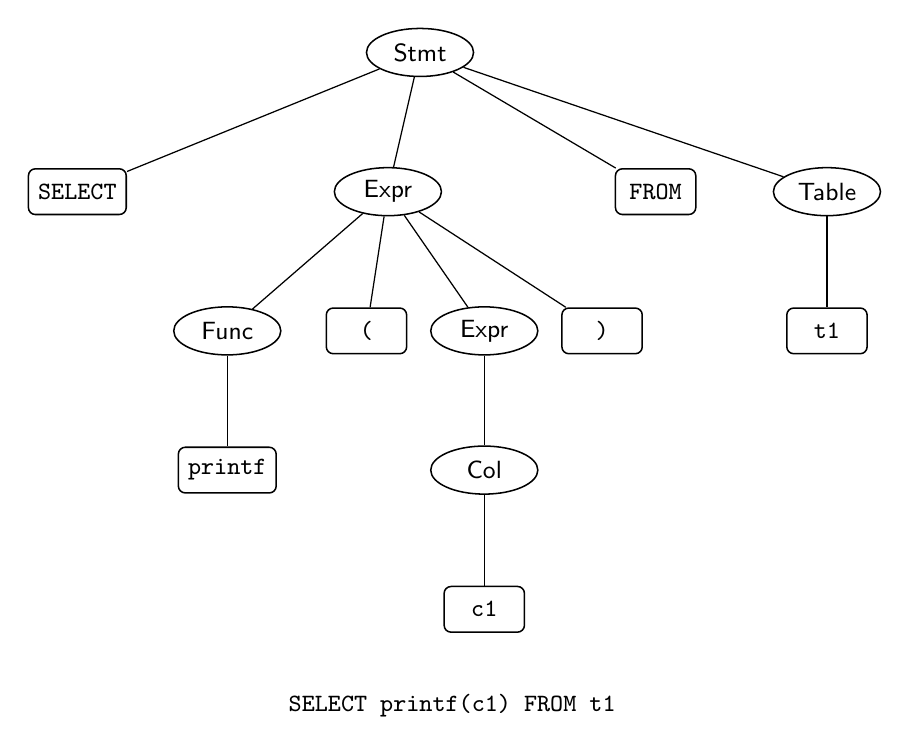
\begin{tikzpicture}[
    x=13.6mm, y=13.6mm,
    every node/.style={font=\small},
    nt/.style={ellipse, draw=black, line width=0.55pt,
        inner xsep=3pt, inner ysep=2pt, font=\small\sffamily,
        minimum width=13.6mm, minimum height=6.1mm},
    lf/.style={rectangle, rounded corners=2.5pt, draw=black, line width=0.55pt,
        inner xsep=3.5pt, inner ysep=2pt, font=\small\ttfamily,
        minimum width=10.2mm, minimum height=5.8mm},
    te/.style={draw=black, line width=0.45pt},
]
    % Level 0
    \node[nt] (root) at (0,0) {Stmt};

    % Level 1
    \node[lf] (sel)   at (-3.2,-1.3) {SELECT};
    \node[nt] (expr1) at (-0.3,-1.3) {Expr};
    \node[lf] (from)  at (2.2,-1.3)  {FROM};
    \node[nt] (tab)   at (3.8,-1.3)  {Table};

    % Level 2
    \node[nt] (func)  at (-1.8,-2.6)  {Func};
    \node[lf] (lpar)  at (-0.5,-2.6) {\textup{(}};
    \node[nt] (expr2) at (0.6,-2.6)  {Expr};
    \node[lf] (rpar)  at (1.7,-2.6)  {\textup{)}};
    \node[lf] (t1)    at (3.8,-2.6)  {t1};

    % Level 3
    \node[lf] (printf) at (-1.8,-3.9) {printf};
    \node[nt] (col)    at (0.6,-3.9)  {Col};

    % Level 4
    \node[lf] (c1) at (0.6,-5.2) {c1};

    % Edges
    \foreach \a/\b in {root/sel, root/expr1, root/from, root/tab,
        expr1/func, expr1/lpar, expr1/expr2, expr1/rpar,
        tab/t1, func/printf, expr2/col, col/c1}
        \draw[te] (\a) -- (\b);

    % Output string
    \node[font=\small\ttfamily, anchor=north] at (0.3,-5.9)
        {SELECT printf(c1) FROM t1};
\end{tikzpicture}
\caption{Derivation tree for \texttt{SELECT printf(c1) FROM t1}.}
\label{fig:derivation-tree}
\end{figure}

The key property for fuzzing is that every string derivable from a well-designed SQL grammar is a syntactically valid SQL statement. By designing the grammar to cover relevant SQL constructs, the generation process is guaranteed to produce inputs that pass the DBMS parser and reach deeper execution stages where vulnerabilities reside.


\section{Fuzzing}
\label{sec:bg-fuzzing}

Fuzzing is an automated technique for discovering software vulnerabilities by generating a large number of inputs, feeding them to a target program, and monitoring for abnormal behavior such as crashes or sanitizer violations~\citep{fuzzingsurvey}. In recent years, fuzzing has been applied extensively to test DBMSs and has found a large number of vulnerabilities~\citep{griffin}.

\paragraph{DBMS fuzzing.}
Unlike fuzzing C libraries that process binary formats, generating high-quality inputs for DBMSs is challenging because DBMSs enforce strict checks on both syntax and semantics~\citep{griffin}. A DBMS first checks the syntactic correctness of a SQL statement; incorrect statements are rejected outright. It then checks the semantics --- for example, whether referenced table and column names actually exist in the database. Statements that fail either check are discarded before reaching the deeper execution logic where vulnerabilities reside~\citep{griffin}.

DBMS fuzzers can be broadly categorized as generation-based or mutation-based~\citep{griffin}. Generation-based fuzzers construct SQL statements from a formal model of the grammar, such as an abstract syntax tree (AST). For example, SQLsmith~\citep{sqlsmith} introspects the database schema to generate type-correct queries, and SQLancer~\citep{sqlancer} generates queries designed to detect logic bugs through differential oracles. Mutation-based fuzzers modify existing SQL statements to produce new test cases, typically building a custom SQL parser and AST mutator for each target DBMS dialect. Squirrel~\citep{squirrel}, for instance, parses SQL into an intermediate representation that preserves semantic relationships, enabling type-aware mutations with coverage feedback.

\paragraph{Coverage-guided greybox fuzzing.}
A central insight of modern fuzzing is the use of code coverage as feedback to guide input generation. Coverage-guided greybox fuzzing, pioneered by AFL~\citep{afl}, instruments the target program to record which code edges (basic block transitions) are exercised during execution. The coverage information is stored in a shared memory bitmap. After executing a test input, the fuzzer checks whether any previously unseen edges were discovered; if so, the input is retained in the corpus for further mutation, otherwise it is discarded~\citep{fuzzingsurvey}. This feedback loop transforms fuzzing from random input generation into a directed search that progressively explores deeper program logic.

The AFL fork server model provides an efficient execution mechanism: rather than creating a new process for each test input, the target program is loaded once, and child processes are created via \texttt{fork()} for each test case. The child inherits the initialized program state, executes the input, and exits. This amortizes startup overhead and isolates crashes --- when a child triggers a fault, the parent remains unaffected~\citep{afl}.

\paragraph{Grammar-based greybox fuzzing.}
General-purpose greybox fuzzers such as AFL are effective for binary formats but struggle with structured inputs like SQL, because random byte-level mutations overwhelmingly produce parser-rejected inputs~\citep{nautilus}. Grammar-based fuzzing addresses this by generating inputs from a context-free grammar (Section~\ref{sec:bg-cfg}), ensuring syntactic validity. Combining grammar-based generation with coverage-guided feedback yields a \textit{grammar-based greybox fuzzer}: a system that generates syntactically valid inputs and uses coverage feedback to steer generation toward unexplored program regions. Nautilus~\citep{nautilus} is the first fuzzer to implement this combination, maintaining a corpus of derivation trees rather than flat strings and applying tree-level mutations guided by edge coverage. Nautilus discovered 13 previously unknown bugs across four interpreter targets (mruby, PHP, ChakraCore, and Lua), of which six were assigned CVEs, demonstrating that the grammar-plus-feedback combination significantly outperforms either approach alone.


\section{Existing Solutions}
\label{sec:bg-related}

Several lines of research address the challenge of testing software that processes structured inputs. This section reviews the most relevant approaches and positions DBMS-Nautilus relative to each.

\paragraph{Generation-based fuzzers.}
CSmith~\citep{csmith} generates random C programs that avoid undefined behavior, enabling differential testing across compilers. CSmith demonstrates that grammar-driven generation can discover deep bugs that mutation-based tools miss, but it operates without coverage feedback: each generated program is independent of all previous executions. LangFuzz~\citep{langfuzz} combines grammar-based generation with code fragments parsed from an existing corpus to fuzz JavaScript interpreters, producing inputs that are both syntactically valid and semantically plausible. However, LangFuzz requires a pre-existing corpus and does not use coverage feedback. IFuzzer~\citep{ifuzzer} applies genetic programming to evolve JavaScript programs that maximize coverage, but evaluates fitness per generation rather than per input. Skyfire~\citep{skyfire} learns a probabilistic context-sensitive grammar from seed inputs and uses it to generate diverse seeds for downstream fuzzers, serving as a seed generator rather than a standalone fuzzer.

\paragraph{DBMS-specific testing tools.}
SQLsmith~\citep{sqlsmith} generates random SQL queries by introspecting database schema metadata, producing type-correct queries with valid table and column references. However, SQLsmith operates without coverage feedback and without weighted sampling over its query templates. Squirrel~\citep{squirrel} introduces an intermediate representation for SQL that encodes semantic relationships, enabling type-aware mutations with coverage feedback. However, Squirrel requires a custom IR parser for each SQL dialect and does not support weighted sampling over structural patterns. SQLancer~\citep{sqlancer} takes a different approach: rather than searching for crashes, it generates queries and checks whether the DBMS returns correct results. NoREC~\citep{norec} and TLP~\citep{tlp} extend this differential testing methodology. These tools are effective at detecting logic bugs (incorrect query results) but do not target memory safety violations, which require a crash-based oracle.

\paragraph{Grammar-based greybox fuzzers.}
Nautilus~\citep{nautilus} was the first to combine grammar-based generation with coverage feedback, discovering 13 bugs (six CVEs) across four interpreter targets. However, Nautilus uses a general-purpose grammar with uniform sampling: all production rules have equal probability, with no mechanism to bias generation toward specific vulnerability classes.

\paragraph{Positioning of DBMS-Nautilus.}
DBMS-Nautilus extends the Nautilus architecture with three domain-specific enhancements. First, the grammar is designed around structural primitives extracted from CVE root-cause analysis, encoding the SQL constructs that stress vulnerability-prone code paths. Second, production rules carry numeric weights that bias sampling toward vulnerability-relevant constructs. Third, the grammar generates self-contained SQL programs from an empty database, eliminating the need for a pre-populated schema. Table~\ref{tab:related-comparison} summarizes the key differences; a checkmark indicates the tool supports the feature and a cross indicates it does not; ``SQL-specific'' indicates whether the tool is specifically designed for SQL or DBMS testing.

\begin{table}[htbp]
\caption{Comparison of DBMS-Nautilus with related fuzzing tools.}
\label{tab:related-comparison}
\centering
\small
\resizebox{\textwidth}{!}{%
\begin{tabular}{lccccc}
\toprule
\textbf{Tool} & \textbf{Grammar} & \textbf{Feedback} & \textbf{Corpus-free} & \textbf{SQL-specific} & \textbf{Weighted} \\
\midrule
AFL~\citep{afl}           & $\times$ & \checkmark & $\times$ & $\times$ & $\times$ \\
CSmith~\citep{csmith}     & \checkmark & $\times$ & \checkmark & $\times$ & $\times$ \\
SQLsmith~\citep{sqlsmith}  & \checkmark & $\times$ & $\times$ & \checkmark & $\times$ \\
Squirrel~\citep{squirrel}  & \checkmark & \checkmark & $\times$ & \checkmark & $\times$ \\
Nautilus~\citep{nautilus}  & \checkmark & \checkmark & \checkmark & $\times$ & $\times$ \\
DBMS-Nautilus             & \checkmark & \checkmark & \checkmark & \checkmark & \checkmark \\
\bottomrule
\end{tabular}}
\end{table}
\newpage\cleardoublepage
\chapter{Proposed Method}
\label{chap:method}

As discussed in Chapter~\ref{chap:background}, byte-level fuzzers cannot effectively test database engines because random mutations produce parser-rejected inputs that never reach deep program logic. Grammar-based fuzzers solve the syntactic validity problem but treat all SQL constructs equally, with no knowledge of which structural patterns are most likely to trigger vulnerabilities. Motivated by this observation, this chapter presents DBMS-Nautilus, a grammar-based greybox fuzzing system that combines Nautilus-style coverage-guided generation~\citep{nautilus} with a domain-specific SQL grammar engineered to target vulnerability-triggering code paths in SQLite. What makes DBMS-Nautilus different from existing fuzzers is its grammar --- the grammar determines what the fuzzer can discover; the fuzzing engine navigates within that space but cannot expand it.

Section~\ref{sec:overview} provides a high-level overview of the system and its components. Section~\ref{sec:grammar-design} presents the grammar design methodology, which constitutes the core contribution of this work. The grammar contains 520 production rules (526 with RQ1 seed rules) organized into a two-layer architecture, designed through root-cause analysis of known CVEs and guided by experimental feedback from fuzzing campaigns.

\section{System Overview}
\label{sec:overview}

DBMS-Nautilus is a grammar-based greybox fuzzer designed specifically for database engines. It combines the coverage-guided fuzzing loop of Nautilus~\citep{nautilus} with a domain-specific SQL grammar that encodes structural attack patterns associated with known vulnerability classes. Existing SQL fuzzers such as SQLsmith~\citep{sqlsmith} generate random queries against a pre-populated database, while Squirrel~\citep{squirrel} maintains an internal schema model to ensure semantic validity. DBMS-Nautilus takes a different approach: the grammar itself generates complete, self-contained SQL programs that create their own schema, populate data, and issue queries --- all starting from an empty in-memory database. This self-contained design means every test case is independently reproducible, requires no external database state, and can be replayed in isolation for crash confirmation.

The system consists of twelve components organized into a closed feedback loop, illustrated in Figure~\ref{fig:architecture}.

\begin{figure}[htbp]
\centering
\makebox[\textwidth][c]{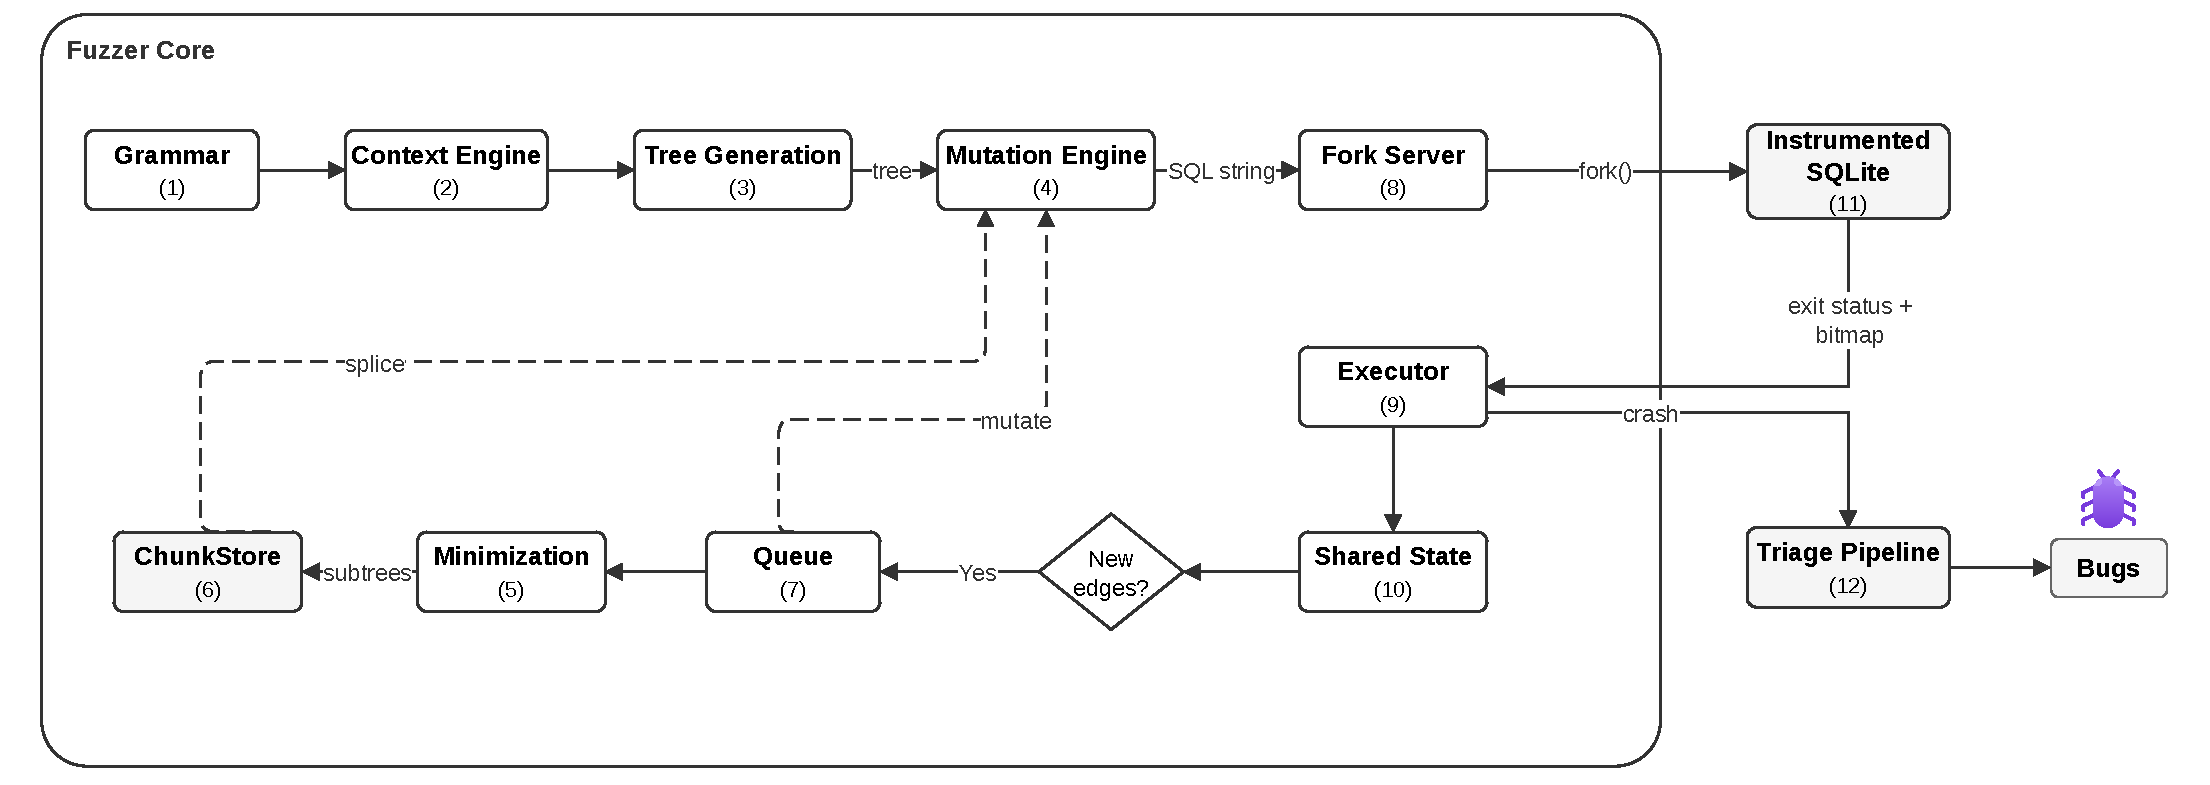
\includegraphics[width=1.25\textwidth]{figures/fig_3_1_architecture.pdf}}
\caption{Architecture of DBMS-Nautilus.}
\label{fig:architecture}
\end{figure}

Components~1 through~10 form the fuzzer core. The data flows as follows: the grammar~(1), a Python script defining 520 weighted production rules, is loaded into the context engine~(2), which stores the rules and performs weighted random selection among applicable alternatives at each non-terminal expansion. Tree generation~(3) uses the context engine to construct complete derivation trees rooted at the start symbol. These trees are either used directly (for initial seed generation) or passed through the mutation engine~(4), which applies five structural mutation operators to create variant inputs. Each mutated tree is unparsed into a SQL string and passed to the fork server~(8), which writes the SQL to a temporary file and forks a child process of the instrumented SQLite binary~(11). The child executes the SQL and exits; the fuzzer executor~(9) reads the shared memory coverage bitmap and the exit status. If the input triggered previously unseen control-flow edges, the tree is added to the queue~(7) for further mutation; if the exit indicates a crash (ASan, UBSan, or signal), the input is saved for triage. The queue manages inputs through a three-state pipeline (Init$\to$Det$\to$Random): during Init, minimization~(5) shrinks the tree while preserving its coverage contribution, and the minimized subtrees are added to the chunk store~(6) for use by splice mutations. During Det and Random, the mutation operators are applied systematically. Shared state~(10) maintains the global coverage bitmap and execution counters across all threads. After a campaign completes, the triage pipeline~(12) processes the collected crashes to deduplicate bugs and match them against known CVEs. The following sections describe each subsystem in detail.

\section{Grammar Engine}
The grammar engine defines the space of SQL inputs that the fuzzer can produce. It loads a context-free grammar specification written as a Python script, where each production rule maps a non-terminal to a string pattern containing terminal symbols and references to other non-terminals. Rules can carry numeric weights that bias the sampling distribution: at each expansion step, the engine selects among applicable rules with probability proportional to their weights, allowing the grammar designer to make certain SQL constructs more likely to appear than others. The grammar engine is the component that distinguishes DBMS-Nautilus from general-purpose grammar fuzzers: by encoding SQL-specific structural patterns and weighting them toward vulnerability-relevant constructs, it concentrates the fuzzer's effort on the most productive regions of the input space. Section~\ref{sec:grammar-design} describes the grammar design methodology in detail.

\section{Generation and Mutation}
The generation and mutation module transforms grammar rules into concrete SQL strings. On each iteration, it either builds a fresh derivation tree by expanding non-terminals according to the grammar, or takes an existing tree from the queue and applies one of five structural mutations: deterministic rule substitution (trying every alternative production at a given node), random subtree regeneration (replacing a subtree with a fresh derivation from the grammar), random recursion expansion (repeating recursive productions to increase nesting depth), splice mutation (replacing a subtree with a fragment of the same non-terminal from the chunk store), or bulk random havoc (applying repeated random subtree replacements in succession). The result is unparsed into a SQL string by reading leaf nodes left to right. This tree-level approach ensures that every generated input is syntactically valid with respect to the grammar, avoiding the wasted executions that plague byte-level mutators when applied to structured languages like SQL.

Figures~\ref{fig:mut-minimize} through~\ref{fig:mut-splice} illustrate minimization and four of the five mutation operators using SQL derivation tree examples. The fifth, bulk random havoc, applies multiple random subtree replacements in succession and is not illustrated separately.

\needspace{12\baselineskip}
In Figure~\ref{fig:mut-minimize}, the \texttt{Expr} subtree \texttt{a + b} is replaced with the smallest valid derivation of the same non-terminal (\texttt{Expr} $\to$ \texttt{Col} $\to$ \texttt{a}), producing a shorter input that preserves the same coverage bits. Subtree minimization is applied immediately after a new coverage-increasing input is discovered. The algorithm iterates over every non-terminal node in the tree and attempts to replace it with the shortest possible subtree for that non-terminal. If the replacement still triggers the same new coverage edges, the shorter tree is kept. This process reduces the tree size without losing the coverage contribution, making subsequent mutations more efficient by operating on a smaller, more focused input.
\vspace{-2mm}
\begin{figure}[H]
\centering
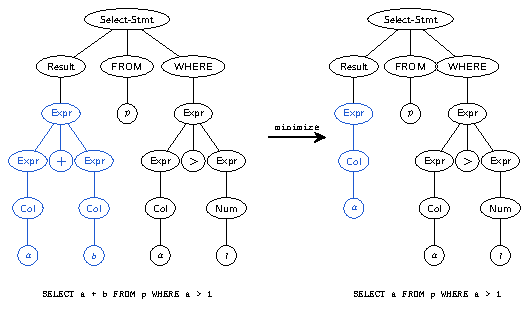
\includegraphics[width=\textwidth]{figures/mutations/fig_3_mutation_minimize.pdf}
\vspace{-3mm}
\caption{Subtree minimization.}
\label{fig:mut-minimize}
\end{figure}
\vspace{-2mm}

\needspace{12\baselineskip}
In Figure~\ref{fig:mut-rules}, the targeted \texttt{Expr} node is systematically replaced with every alternative production rule for that non-terminal, generating one mutant per rule. This deterministic mutation ensures that every possible alternative for a given non-terminal is explored at least once. For example, if \texttt{Expr} has four production rules, this operator generates four distinct mutants from a single parent tree. This exhaustive exploration is particularly valuable in the early stages of fuzzing (the Det phase), where the goal is to rapidly cover all syntactic alternatives before switching to random mutations.
\vspace{-2mm}
\begin{figure}[H]
\centering
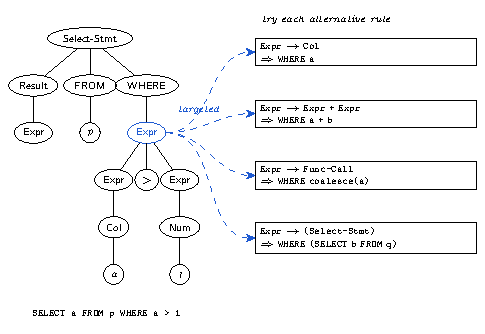
\includegraphics[width=\textwidth]{figures/mutations/fig_3_mutation_rules.pdf}
\vspace{-3mm}
\caption{Deterministic rule substitution (\texttt{mut\_rules}).}
\label{fig:mut-rules}
\end{figure}
\vspace{-2mm}

\needspace{14\baselineskip}
In Figure~\ref{fig:mut-random}, a randomly selected node's subtree is replaced with a fresh derivation from the grammar; the comparison \texttt{a > 1} is replaced with a subquery \texttt{a IN (SELECT b FROM q)}. Unlike deterministic rule substitution, which tries every alternative at a fixed node, random subtree regeneration picks both the target node and the replacement randomly. The size of the new subtree is bounded by the configured maximum tree size (set to 300 nodes in our experiments). This mutation is the primary source of structural diversity: it can introduce entirely new SQL constructs into an existing tree, such as replacing a simple comparison with a correlated subquery or a window function call.
\vspace{-2mm}
\begin{figure}[H]
\centering
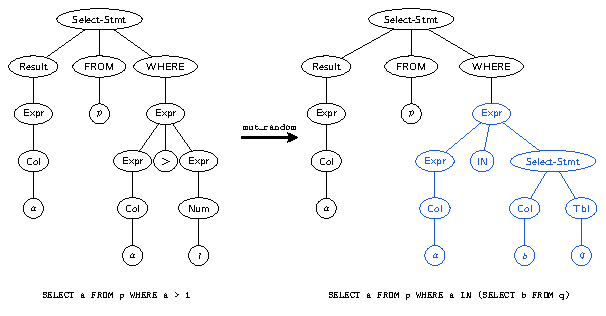
\includegraphics[width=\textwidth]{figures/mutations/fig_3_mutation_random.pdf}
\vspace{-3mm}
\caption{Random subtree regeneration (\texttt{mut\_random}).}
\label{fig:mut-random}
\end{figure}
\vspace{-2mm}

\needspace{12\baselineskip}
In Figure~\ref{fig:mut-recursion}, a recursive production (\texttt{Expr} $\to$ \texttt{Expr + Expr}) is repeated multiple times, increasing expression nesting depth. The repetition count is controlled by a randomly chosen node budget of $2 \cdot 2^k$ nodes where $k$ is chosen uniformly from $\{1, 2, \ldots, 10\}$, giving budgets from 4 to 2048; the actual number of repetitions is the budget divided by the size of the recursive structure. This mutation only expands; collapsing is performed by minimization. Deep nesting is important for vulnerability discovery because SQLite processes recursive SQL structures (nested expressions, subqueries, compound operators) through stack-based evaluation, and excessive depth can trigger stack overflows, integer overflows in intermediate computations, or null pointer dereferences when internal limits are exceeded.
\vspace{-2mm}
\begin{figure}[H]
\centering
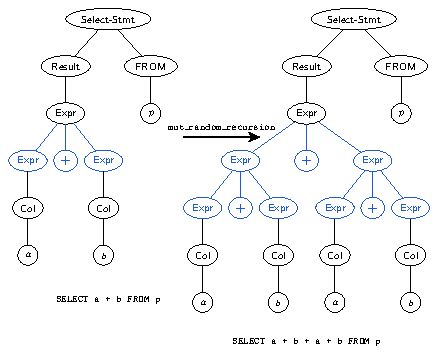
\includegraphics[width=\textwidth]{figures/mutations/fig_3_mutation_recursion.pdf}
\vspace{-3mm}
\caption{Random recursion expansion (\texttt{mut\_random\_recursion}).}
\label{fig:mut-recursion}
\end{figure}
\vspace{-2mm}

\needspace{14\baselineskip}
In Figure~\ref{fig:mut-splice}, a subtree from the ChunkStore (populated by minimized interesting inputs) replaces a compatible node in the current tree, matched by non-terminal: an \texttt{Expr} node producing \texttt{a > 1} is replaced with an \texttt{Expr} node producing \texttt{printf('\%.*g', 2147483647, 0.01)}. Splice mutation is the key mechanism for combining structural patterns discovered in separate executions. When one input discovers a new code path through a particular SQL construct, minimization extracts the relevant subtree and stores it in the ChunkStore. Splice then transplants that subtree into other inputs, creating new combinations that neither parent input could produce alone. This cross-pollination is how the fuzzer discovers bugs that require multiple structural patterns to co-occur in a single input.
\vspace{-2mm}
\begin{figure}[H]
\centering
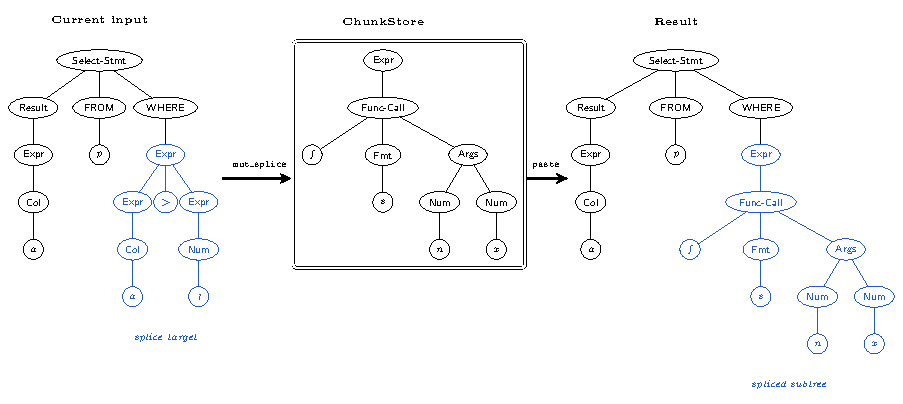
\includegraphics[width=\textwidth]{figures/mutations/fig_3_mutation_splice.pdf}
\vspace{-3mm}
\caption{Splice mutation (\texttt{mut\_splice}).}
\label{fig:mut-splice}
\end{figure}

\section{Fork Server and Harness}
The fork server and harness form the execution layer that runs each generated SQL input against a real SQLite build. The harness opens an empty in-memory SQLite database, then uses the AFL fork-server protocol~\citep{afl} to efficiently create a child process for each test case without the overhead of full process initialization. Each child executes one SQL input and exits. SQLite is compiled with AddressSanitizer (ASan) and UndefinedBehaviorSanitizer (UBSan) instrumentation, which act as oracles: ASan detects memory safety violations such as buffer overflows and use-after-free, while UBSan detects undefined behavior such as integer overflow and null pointer dereference. Without these sanitizers, many vulnerabilities would execute silently without any observable failure.

\section{Coverage Feedback and Queue}
The coverage feedback mechanism is what makes DBMS-Nautilus a \textit{greybox} fuzzer rather than a purely generative one. After each execution, the fuzzer checks whether the input exercised any previously unseen control-flow edges in SQLite by comparing the execution's coverage bitmap against the global bitmap. If new edges are found, the input is verified for deterministic behavior (re-executed five times to confirm the new edges are reproducible) and then classified as \textit{interesting} and added to the queue. The queue uses a three-state pipeline adapted from Nautilus: each input progresses through Init (minimization), Det (deterministic rule substitution plus random mutations), and Random (random mutations only). The original Nautilus uses a four-state pipeline that includes an additional \texttt{detafl} stage for AFL-style byte-level mutations; DBMS-Nautilus omits this stage because byte-level mutations (bit flips, arithmetic increments) produce parser-rejected SQL inputs that waste execution budget without reaching deep program logic. Over time, the feedback loop steers generation toward unexplored program regions, progressively expanding coverage into deeper and more complex code paths. Without coverage feedback, the fuzzer would generate inputs uniformly from the grammar with no awareness of which inputs are actually reaching new code --- a strictly less efficient strategy, as the experiments in Chapter~\ref{chap:experiments} demonstrate.

\section{Triage Pipeline}
The triage pipeline operates after a fuzzing campaign completes. It processes the collected crashing inputs to determine how many distinct bugs were found, whether any correspond to known CVEs, and how reliably each crash reproduces. This post-campaign analysis transforms raw crash data into actionable vulnerability reports. Chapter~\ref{chap:experiments} describes the triage methodology in detail.

\section{Self-Contained Test Cases}
A key design decision is that every test case begins from an empty database. The grammar generates multi-statement SQL programs that first create tables and insert data (via the \texttt{Schema-Setup} non-terminal), then issue the queries that exercise the target code paths. This contrasts with SQLsmith, which requires a pre-populated database and introspects its schema at runtime, and Squirrel, which maintains an evolving schema model during fuzzing. The self-contained approach has three advantages: the harness requires no setup beyond opening an empty database, every crashing input can be replayed in isolation without reconstructing external state, and the grammar retains full control over which schema patterns appear in each test case. Between schema creation and query execution, an \texttt{Insert-Stmt} non-terminal generates INSERT statements that populate the created tables with random rows, ensuring that subsequent queries operate on non-empty data and exercise the full execution path through SQLite's query engine. The Schema-Setup$\to$Insert-Stmt$\to$Stress-Query ordering within each generated program ensures referential consistency: tables and columns exist and contain data before they are queried. Remaining semantic errors (e.g., type mismatches in expressions) are handled gracefully by SQLite's error-tolerant execution --- they produce error return codes rather than crashes, and are thus filtered out naturally by the crash-detection oracle.

Table~\ref{tab:components} groups the twelve components into five functional subsystems, showing their implementation languages and roles in the pipeline. The components are grouped by functional subsystem with implementation sizes; components (1--12) correspond to Figure~\ref{fig:architecture}. The Grammar Spec.\ row refers to the grammar specification loaded at startup.

\begin{table}[htbp]
\caption{DBMS-Nautilus system components.}
\label{tab:components}
\centering
\footnotesize
\resizebox{\textwidth}{!}{%
\begin{tabular}{lllrl}
\toprule
\textbf{Subsystem} & \textbf{Lang.} & \textbf{Module} & \textbf{LoC} & \textbf{Key Responsibility} \\
\midrule
Grammar Spec.\ (1) & Python & \texttt{grammars/} & 840 & 520 weighted production rules \\
Context Engine (2) & Rust & \texttt{grammartec/} & \multirow{5}{*}{2{,}466} & Rule storage, weighted selection \\
Tree Generation (3) & Rust & \texttt{grammartec/} & & Derivation tree construction \\
Mutation Engine (4) & Rust & \texttt{grammartec/} & & 5 structural mutation operators \\
Minimization (5) & Rust & \texttt{grammartec/} & & Shrink trees preserving coverage \\
ChunkStore (6) & Rust & \texttt{grammartec/} & & Index subtrees ($\leq$30 nodes) for splice \\
\midrule
Queue (7) & Rust & \texttt{fuzzer/} & \multirow{3}{*}{2{,}384} & Three-state pipeline (Init$\to$Det$\to$Random) \\
Fuzzer Executor (9) & Rust & \texttt{fuzzer/} & & Per-thread coordination, dedup \\
Shared State (10) & Rust & \texttt{fuzzer/} & & Global bitmap, counters \\
\midrule
Fork Server (8) & Rust & \texttt{forksrv/} & 426 & AFL protocol, shared memory bitmap \\
Harness & C & \texttt{harness/} & 89 & Empty DB, \texttt{\_\_AFL\_INIT()}, one-exec-per-fork \\
\midrule
Triage Pipeline (12) & Python & \texttt{triage/} & 884 & Stack dedup, CVE matching, fidelity scoring \\
\bottomrule
\end{tabular}}
\end{table}


%% ====================================================================
\section{Grammar Design}
\label{sec:grammar-design}
%% ====================================================================

What makes DBMS-Nautilus different is its grammar. This grammar encodes SQL structural attack patterns that trigger vulnerability classes rather than specific proof-of-concept inputs. This ``zero PoC contamination'' principle ensures that the fuzzer discovers bugs through compositional exploration rather than replaying known attacks.

To illustrate, consider CVE-2020-9327~\citep{cve20209327}, a null pointer dereference in SQLite's generated column processor. Listing~\ref{lst:cve9327-poc} shows the original proof-of-concept from the SQLite bug tracker~\citep{cve20209327ticket}.

\begin{lstlisting}[caption={Original PoC for CVE-2020-9327.}, label={lst:cve9327-poc}, basicstyle=\ttfamily\small, numbers=none, frame=single, xleftmargin=1cm, xrightmargin=1cm]
CREATE TABLE v0(v3, v1 AS(v1) UNIQUE);
CREATE TABLE v5(v6 UNIQUE, v7 UNIQUE);
CREATE VIEW v8(v9) AS
  SELECT coalesce(v3, v1) FROM v0
  WHERE v1 IN('MED BOX');
SELECT * FROM v8 JOIN v5
  WHERE 0 > v7 AND v9 OR v6 = 's%';
\end{lstlisting}

Rather than encoding this PoC as a fixed string, the grammar decomposes it into independent, composable production rules. Table~\ref{tab:poc-decomposition} shows how each PoC element maps to a grammar rule.

\begin{table}[htbp]
\caption{Decomposition of CVE-2020-9327 PoC into grammar rules.}
\label{tab:poc-decomposition}
\centering
\scriptsize
\begin{tabular}{>{\raggedright\arraybackslash}p{2.8cm}>{\raggedright\arraybackslash}p{4.2cm}>{\raggedright\arraybackslash}p{5.8cm}}
\toprule
\textbf{\footnotesize Description} & \textbf{\footnotesize PoC SQL} & \textbf{\footnotesize Grammar Production Rule} \\
\midrule
Self-referential generated column &
  \texttt{CREATE TABLE v0(v3, v1 AS(v1) UNIQUE)} &
  \textit{Schema-Setup} $\to$ \texttt{CREATE TABLE IF NOT EXISTS p(\{Col-Def-List-GenCol\})} \newline
  \textit{Col-Def-List-GenCol} $\to$ \texttt{a \{Type-Name\}, b AS(b) UNIQUE} \\
\midrule
View wrapping the query &
  \texttt{CREATE VIEW v8(v9) AS SELECT coalesce(v3, v1) FROM v0 WHERE v1 IN('MED BOX')} &
  \textit{Schema-Setup} $\to$ \texttt{CREATE TABLE ...; CREATE VIEW IF NOT EXISTS v1 AS \{Select-Stmt\}} \\
\midrule
\texttt{coalesce()} forcing evaluation &
  \texttt{coalesce(v3, v1)} &
  \textit{Func-Call} $\to$ \texttt{coalesce(\{Expr\}, \{Expr\})} \\
\midrule
JOIN combining view with table &
  \texttt{SELECT * FROM v8 JOIN v5 WHERE 0 > v7 AND v9 OR v6 = 's\%'} &
  \textit{Stress-Query} $\to$ \texttt{SELECT \{Result-Col-List\} FROM \{Table-Name\} NATURAL JOIN \{Table-Name\} WHERE \{Expr\}} \\
\bottomrule
\end{tabular}
\end{table}

No single grammar rule produces the complete PoC. The fuzzer must independently select a schema with generated columns, a view definition, a \texttt{coalesce} expression, and a JOIN-based query --- then compose them into a single valid SQL program. The crash is only triggered when the correct combination emerges from this compositional space.

This design philosophy yields three constraints:

\begin{enumerate}[label=(\alph*)]
    \item No grammar rule may contain a complete CVE proof-of-concept as a fixed string.
    \item Every structural pattern needed to reach a target CVE must exist as a composable non-terminal.
    \item The grammar must preserve sufficient compositional freedom to discover novel combinations beyond the known CVEs.
\end{enumerate}

A natural concern is circularity: the grammar is informed by CVE root-cause analysis, and the evaluation measures CVE rediscovery. This is by design --- known CVEs serve as ground truth. The zero PoC contamination principle (constraint~a) ensures that rediscovery is not trivial: the grammar provides structural building blocks, and the fuzzer must compose them correctly from a large combinatorial space. Chapter~\ref{chap:experiments} further validates the methodology by showing that the grammar also discovers bugs beyond the known CVEs.

In its final form, the base grammar contains 520 production rules: 471 in Layer~1 (SQL atoms) and 49 in Layer~2 (composed vulnerability-targeting shapes). For the RQ1 CVE rediscovery evaluation (Chapter~\ref{chap:experiments}), six low-weight seed rules are added, bringing the total to 526. The complete grammar specification is available in the project repository as a Python script.

\subsection{Two-Layer Architecture}
\label{sec:layer-decomposition}

A SQL statement that triggers a vulnerability is never a single construct --- it is a combination of a schema definition, a query pattern, and sometimes a boundary-value function call. To capture this compositional structure, the grammar separates concerns into two layers: Layer~1 provides the vocabulary (what SQL constructs exist), and Layer~2 provides the sentences (how those constructs combine into vulnerability-triggering patterns). This separation means that adding a new SQL construct to Layer~1 automatically makes it available to all Layer~2 patterns, and adding a new Layer~2 pattern immediately benefits from all existing Layer~1 constructs.

\paragraph{Layer 1: SQL Atoms (471 rules).}
Layer~1 defines the individual SQL constructs that serve as building blocks. Table~\ref{tab:layer1-categories} groups them by category. For example, the \texttt{Expr} non-terminal has over 30 alternatives --- including arithmetic (\texttt{a + b}), comparison (\texttt{a > 1}), function calls (\texttt{coalesce(a, b)}), subqueries (\texttt{(SELECT ...)}), and window functions (\texttt{SUM(c) OVER()}). Similarly, \texttt{Col-Def} can produce a regular column (\texttt{a INTEGER}), a generated column (\texttt{b AS(b) UNIQUE}), or a column with constraints (\texttt{c TEXT NOT NULL}). Each Layer~1 rule produces a syntactically valid SQL fragment; Layer~2 composes these fragments into complete statements.

\begin{table}[htbp]
\caption{Layer~1 non-terminal categories.}
\label{tab:layer1-categories}
\centering
\small
\resizebox{\textwidth}{!}{%
\begin{tabular}{lrl}
\toprule
\textbf{Category} & \textbf{Rules} & \textbf{Examples} \\
\midrule
Expressions       & 30+ & arithmetic, comparison, subquery, window function \\
Clauses           & 20+ & SELECT, FROM, WHERE, JOIN, GROUP BY, HAVING \\
DDL statements    & 15+ & CREATE TABLE, VIEW, INDEX, TRIGGER \\
DML statements    & 10+ & INSERT, UPDATE, DELETE \\
Function calls    & 15+ & aggregate, scalar, window-specific, coalesce \\
Terminal literals  & 20+ & integers, boundary values, strings, blobs \\
Column definitions & 10+ & regular, generated (STORED/VIRTUAL), constrained \\
\bottomrule
\end{tabular}}
\end{table}

\paragraph{Layer 2: Composed Shapes (49 rules).}
Layer~2 composes Layer~1 atoms into four high-level shapes that target specific vulnerability classes. Each shape is a non-terminal whose production rules define complete SQL statement patterns. Figure~\ref{fig:two-layer} illustrates the composition hierarchy.

Every generated SQL program begins from the start symbol \texttt{Sql-Stmt}, which selects:
\begin{itemize}
    \item \texttt{Schema-Setup} (6 alternatives) --- creates the database schema. Appears in three of the four \texttt{Sql-Stmt} alternatives.
    \item \texttt{Stress-Query} (8 alternatives) --- issues a query exercising a specific code path in SQLite's query planner. Appears in two of four alternatives.
    \item \texttt{Boundary-Func-Call} (7 alternatives) --- calls a function with boundary-value arguments. Appears in one standalone alternative.
    \item \texttt{Validation-Op} (4 alternatives) --- runs a PRAGMA or consistency check. Appears in one alternative.
\end{itemize}

\noindent The required shapes appear in every generated statement. The optional shapes are selected by weighted sampling --- their probability of inclusion is controlled by their production rule weights. This means the fuzzer samples from the Cartesian product of all Layer~2 shapes: for example, a single input might combine a generated-column schema, a NATURAL JOIN query, and a \texttt{printf} boundary call, simultaneously exercising SQLite's column resolver, join optimizer, and string formatting implementation.

\begin{figure}[htbp]
\centering
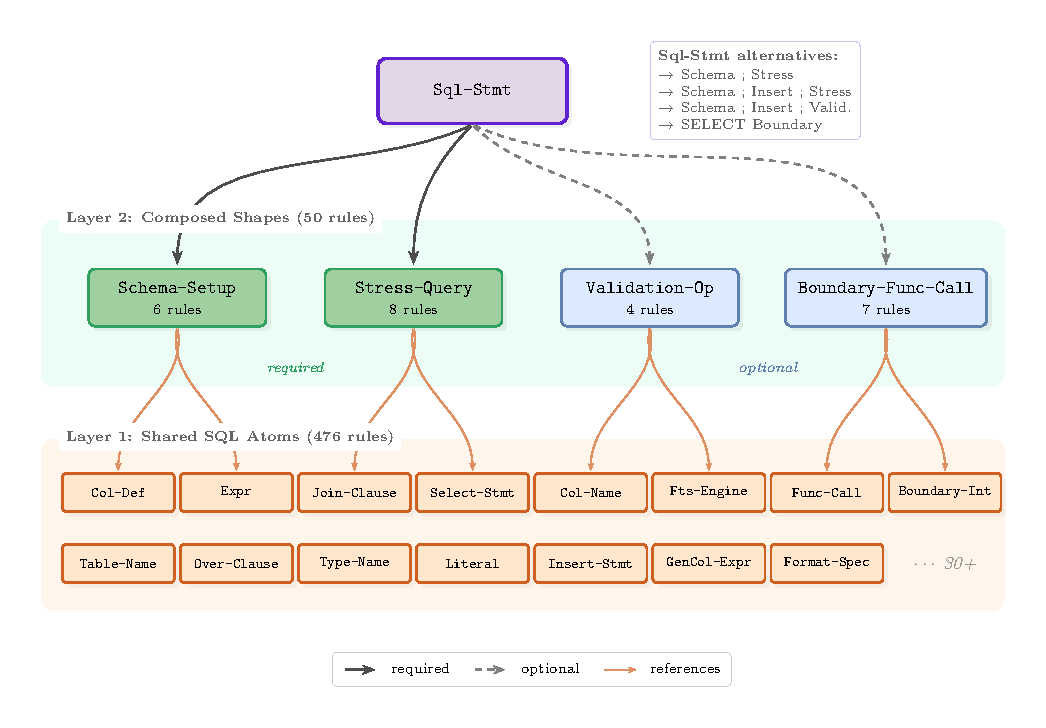
\includegraphics[width=\textwidth]{figures/fig_3_2_grammar_layers.pdf}
\caption{Two-layer grammar architecture.}
\label{fig:two-layer}
\end{figure}

\subsection{Structural Pattern Categories}
\label{sec:pattern-categories}

Each of the four Layer~2 shapes targets a distinct SQLite subsystem where vulnerabilities cluster. The categorization follows from root-cause analysis of known CVEs: each vulnerability implicates specific SQLite internals, and the grammar encodes the SQL constructs that exercise those internals. This section describes each category: what it targets, why bugs occur there, and what the grammar rules look like.

\paragraph{Schema Topology Patterns.}
The schema determines which SQLite subsystems are activated before any query runs. A simple \texttt{CREATE TABLE} only exercises the table creation code, but a schema with generated columns also activates the generated column processor, and a schema with views activates the view materializer. The \texttt{Schema-Setup} non-terminal provides six alternatives that cover these different topologies. Listing~\ref{lst:schema-setup} shows the complete set.

Why this matters: generated columns are resolved by evaluating arbitrary expressions that may reference other columns in the same table. When a column references itself --- \texttt{b AS(b) UNIQUE} --- the column resolver enters a recursive loop that can read an uninitialized pointer (CVE-2020-9327~\citep{cve20209327}) or loop infinitely (CVE-2019-19646~\citep{cve201919646}). Views add an extra layer of column resolution: the view's SELECT statement must be re-resolved every time the view is queried, creating additional opportunities for null dereferences during column name matching. The relative sampling priority of each alternative reflects how many target CVEs involve that schema shape: generated columns participate in two CVEs, while FTS virtual tables serve primarily as a diversity source.

\begin{lstlisting}[language=Python, caption={Schema-Setup alternatives (Layer 2).}, label=lst:schema-setup, basicstyle=\ttfamily\small, numbers=left]
# S1: Single table, basic columns
ctx.rule("Schema-Setup",
    "CREATE TABLE IF NOT EXISTS p({Col-Def-List})")

# S2: Table with generated column + constraints
ctx.rule("Schema-Setup",
    "CREATE TABLE IF NOT EXISTS p({Col-Def-List-GenCol})")

# S3: Two tables (enables JOINs between p and q)
ctx.rule("Schema-Setup",
    "CREATE TABLE IF NOT EXISTS p({Col-Def-List});\n"
    "CREATE TABLE IF NOT EXISTS q({Col-Def-List})")

# S4: Table + VIEW
ctx.rule("Schema-Setup",
    "CREATE TABLE IF NOT EXISTS p({Col-Def-List});\n"
    "CREATE VIEW IF NOT EXISTS v1 AS {Select-Stmt}")

# S5: Virtual table (FTS5/FTS3)
ctx.rule("Schema-Setup",
    "CREATE VIRTUAL TABLE IF NOT EXISTS fts_t1 "
    "USING {Fts-Engine}({Col-Name-List})")

# S6: Table + INDEX
ctx.rule("Schema-Setup",
    "CREATE TABLE IF NOT EXISTS p({Col-Def-List});\n"
    "CREATE INDEX IF NOT EXISTS idx1 ON p({Col-Name})")
\end{lstlisting}

\paragraph{Query Stress Patterns.}
The query determines which optimizer and execution paths are exercised after the schema is set up. SQLite's query planner performs complex AST transformations --- join reordering, subquery flattening, compound query alignment --- each involving pointer manipulation across multiple table scopes. These transformations are where null dereferences, use-after-free, and off-by-one bugs cluster. The \texttt{Stress-Query} non-terminal provides eight patterns, each targeting a different optimizer path. Table~\ref{tab:stress-query-patterns} summarizes all eight patterns and their target code paths. Listing~\ref{lst:stress-query} shows the complete set of rules.

\begin{table}[H]
\caption{Query stress patterns and their target code paths.}
\label{tab:stress-query-patterns}
\centering
\small
\begin{tabular}{llp{6.5cm}}
\toprule
\textbf{Pattern} & \textbf{SQL Construct} & \textbf{Target Code Path} \\
\midrule
Q1 & SELECT \ldots WHERE & Basic expression evaluation and filtering \\
Q2 & WHERE EXISTS (subquery) & Correlated subquery evaluation \\
Q3 & NATURAL JOIN & Column name matching across tables~\citep{cve202013435} \\
Q4 & WITH RECURSIVE & Recursive CTE expansion with termination detection \\
Q5 & INTERSECT / EXCEPT & Compound query column alignment~\citep{cve202015358, cve202013871} \\
Q6 & Self-JOIN \ldots ON & Join optimizer with aliased self-references \\
Q7 & Nested subqueries & Subquery flattening and derived table handling \\
Q8 & EXPLAIN QUERY PLAN & Plan serialization across full optimized AST \\
\bottomrule
\end{tabular}
\end{table}

For example, NATURAL JOIN (Q3) forces SQLite's column matching algorithm to pair columns across tables by name. When combined with a schema containing generated columns (from Schema Topology), this name-matching process must also resolve the generated column expression --- creating the conditions for the null dereference in CVE-2020-13435~\citep{cve202013435}. Similarly, compound queries with EXCEPT (Q5) force the optimizer to align result columns from independently optimized subqueries, stressing the column-alignment code where CVE-2020-13871~\citep{cve202013871} and CVE-2020-15358~\citep{cve202015358} were found.

\begin{lstlisting}[language=Python, caption={Stress-Query alternatives (Layer 2).}, label=lst:stress-query, basicstyle=\ttfamily\small, numbers=left]
# Q1: Base SELECT (full compositional freedom)
ctx.rule("Stress-Query", "{Select-Stmt}")

# Q2: EXISTS subquery
ctx.rule("Stress-Query",
    "SELECT {Result-Col-List} FROM {Table-Name} "
    "WHERE EXISTS ({Select-Stmt})")

# Q3: NATURAL JOIN
ctx.rule("Stress-Query",
    "SELECT {Result-Col-List} FROM {Table-Name} "
    "NATURAL JOIN {Table-Name} WHERE {Expr}")

# Q4: Recursive CTE
ctx.rule("Stress-Query",
    "WITH RECURSIVE {Cte-Def} "
    "SELECT {Result-Col-List} FROM {Table-Name}")

# Q5: Compound query (INTERSECT/EXCEPT)
ctx.rule("Stress-Query",
    "{Select-Stmt} {Compound-Op} {Select-Stmt}")

# Q6: Self-JOIN + expression
ctx.rule("Stress-Query",
    "SELECT {Result-Col-List} FROM {Table-Name} "
    "JOIN {Table-Name} {Col-Alias} ON {Expr}")

# Q7: Nested subquery chain
ctx.rule("Stress-Query",
    "SELECT {Result-Col-List} FROM "
    "(SELECT {Result-Col-List} FROM {Table-Name} "
    "WHERE {Expr}) AS sub1")

# Q8: EXPLAIN QUERY PLAN
ctx.rule("Stress-Query",
    "EXPLAIN QUERY PLAN {Select-Stmt}")
\end{lstlisting}

\paragraph{Boundary Value Patterns.}
Some SQLite vulnerabilities are triggered not by complex query structures but by specific numeric values that overflow internal integer representations. The \texttt{Boundary-Func-Call} non-terminal combines SQLite built-in functions with boundary-value arguments --- INT32\_MAX (2147483647), INT32\_MAX+1, INT32\_MIN, and INT64\_MAX --- to probe these overflow points. Listing~\ref{lst:boundary-func} shows the seven alternatives across three function families:

\begin{itemize}
    \item \textbf{printf variants} (3 rules): pair format specifiers (\texttt{\%.*g}, \texttt{\%.*f}) with boundary integers. This is how CVE-2020-13434~\citep{cve202013434} is triggered: \texttt{printf('\%.*g', 2147483647, 0.01)} causes an integer overflow in SQLite's string formatting when the width parameter equals INT32\_MAX.
    \item \textbf{substr variants} (2 rules): exercise heap buffer boundaries with boundary-value offsets and lengths, probing the substring implementation's bounds checking.
    \item \textbf{zeroblob/round} (2 rules): \texttt{hex(zeroblob(N))} stresses memory allocation with large $N$; \texttt{round} exercises float-to-int conversion edge cases.
\end{itemize}

\begin{lstlisting}[language=Python, caption={Boundary-Func-Call alternatives.}, label=lst:boundary-func, basicstyle=\ttfamily\small, numbers=left]
ctx.rule("Boundary-Func-Call",
    "printf({Format-Spec}, {Boundary-Int}, {Boundary-Float})")
ctx.rule("Boundary-Func-Call",
    "printf({Format-Spec}, {Boundary-Int})")
ctx.rule("Boundary-Func-Call",
    "printf({Printf-Fmt-Spec}, {Boundary-Int}, {Str-Literal})")
ctx.rule("Boundary-Func-Call",
    "substr({Str-Literal}, {Boundary-Int})")
ctx.rule("Boundary-Func-Call",
    "substr({Str-Literal}, {Boundary-Int}, {Boundary-Int})")
ctx.rule("Boundary-Func-Call",
    "hex(zeroblob({Boundary-Int}))")
ctx.rule("Boundary-Func-Call",
    "round({Boundary-Float}, {Boundary-Int})")

ctx.rule("Format-Spec", "'%.*g'")
ctx.rule("Format-Spec", "'%.*f'")

ctx.rule("Boundary-Int", "2147483647")    # INT32_MAX
ctx.rule("Boundary-Int", "2147483648")    # INT32_MAX+1
ctx.rule("Boundary-Int", "-2147483648")   # INT32_MIN
ctx.rule("Boundary-Int", "9223372036854775807")  # INT64_MAX
\end{lstlisting}

\paragraph{Validation Operations.}
Normal queries exercise SQLite's query planner and execution engine, but some vulnerabilities reside in separate code paths that are only activated by maintenance operations. The \texttt{Validation-Op} non-terminal provides four such operations, shown in Listing~\ref{lst:validation-op}. These operations traverse internal data structures --- B-trees, schema tables, index metadata --- using code paths that are distinct from normal query execution. When the schema contains unusual constructs such as generated columns, these traversals can encounter unexpected states: CVE-2019-19646~\citep{cve201919646} is triggered when \texttt{PRAGMA integrity\_check} encounters a generated column with a NOT NULL constraint, causing an infinite loop in the column validation logic.

\begin{lstlisting}[language=Python, caption={Validation-Op alternatives.}, label=lst:validation-op, basicstyle=\ttfamily\small, numbers=left]
ctx.rule("Validation-Op",
    "PRAGMA integrity_check")
ctx.rule("Validation-Op",
    "PRAGMA quick_check")
ctx.rule("Validation-Op",
    "ANALYZE {Table-Name}")
ctx.rule("Validation-Op",
    "EXPLAIN QUERY PLAN {Select-Stmt}")
\end{lstlisting}

Table~\ref{tab:pattern-subsystem} summarizes the mapping between pattern categories and the SQLite subsystems they exercise. Each category exercises distinct internal code paths where vulnerabilities cluster.

\begin{table}[htbp]
\caption{Structural pattern categories.}
\label{tab:pattern-subsystem}
\centering
\small
\begin{tabular}{>{\raggedright\arraybackslash}p{3.2cm} >{\raggedright\arraybackslash}p{4.0cm} >{\raggedright\arraybackslash}p{5.5cm}}
\toprule
\textbf{Pattern Category} & \textbf{Target Subsystem} & \textbf{Vulnerability Mechanism} \\
\midrule
Schema Topology (S1--S6) & Column resolver, generated column processor, view materializer & Circular dependencies, null dereferences in column resolution \\
Query Stress (Q1--Q8) & Query planner, join optimizer, compound query engine & Name resolution errors, use-after-free in AST transforms \\
Boundary Values & printf, substr, zeroblob implementations & Integer overflow, buffer overread, allocation failures \\
Validation Ops & Integrity checker, B-tree traversal, schema validator & Page cache errors, type checking failures on unusual schemas \\
\bottomrule
\end{tabular}
\end{table}

\subsection{Cross-Pollination of Structural Patterns}
\label{sec:cross-pollination}

A key property of the grammar is that structural patterns are not labeled or isolated per CVE. Each non-terminal encodes a SQL structural affordance --- a syntactic shape that participates in one or more vulnerability-triggering code paths --- without indicating which specific vulnerability it targets. This design choice ensures that the grammar captures \emph{structural categories} of vulnerabilities rather than individual instances, and it produces a cross-pollination effect: a single non-terminal serves multiple CVEs simultaneously, and a single CVE requires patterns drawn from multiple independent non-terminals.

Cross-pollination arises naturally from the independence of Layer~2 selections. On each generated input, the fuzzer independently selects a \texttt{Schema-Setup} variant, a \texttt{Stress-Query} variant, and optionally a \texttt{Boundary-Func-Call} or \texttt{Validation-Op}. Because these selections are governed by independent weighted distributions, the fuzzer samples from the Cartesian product of all Layer~2 shapes --- producing combinations that the grammar designer never explicitly planned. For example, a single generated input might combine S2 (generated columns) with Q3 (NATURAL JOIN) and a printf boundary call, exercising the intersection of SQLite's generated column processor, join optimizer, and printf implementation simultaneously.

Table~\ref{tab:cve-structural} maps each target CVE to the structural patterns required to trigger it. Every CVE requires between two and five patterns drawn from different non-terminal groups. Several key patterns are shared across multiple CVEs: generated columns participate in two CVEs, JOIN patterns serve three, and \texttt{coalesce} appears in two. This sharing means that improving the grammar's ability to reach one CVE simultaneously improves its ability to reach others --- a multiplicative benefit that would not arise if each CVE were targeted by isolated grammar rules.

\begin{table}[htbp]
\caption{Structural patterns required for each target CVE.}
\label{tab:cve-structural}
\centering
\begin{tabular}{lrl}
\toprule
\textbf{CVE} & \textbf{Patterns} & \textbf{Required Structural Elements} \\
\midrule
CVE-2019-19646 & 2 & Generated column, PRAGMA integrity\_check \\
CVE-2020-13434 & 2 & printf() call, INT32 boundary value \\
CVE-2020-9327  & 4 & Generated column, coalesce(), JOIN, CREATE VIEW \\
CVE-2020-13435 & 5 & NATURAL JOIN, coalesce(), window OVER(), \\
               &   & UNIQUE column, IN subquery \\
CVE-2020-13871 & 3 & EXCEPT, multi-column ORDER BY, scalar subquery \\
CVE-2020-15358 & 3 & CREATE VIEW with ORDER BY, INTERSECT, \\
               &   & implicit JOIN (comma-separated FROM) \\
\bottomrule
\end{tabular}
\end{table}

This cross-pollination property has two important consequences. First, any CVE rediscovery constitutes a genuine compositional achievement: the fuzzer must independently select the correct combination of non-terminals from a large combinatorial space, with each selection governed by a weighted probability distribution. Second, the grammar discovers bugs beyond its explicit design targets. The nine non-CVE bug classes reported in Chapter~\ref{chap:experiments} --- including FTS tokenizer null dereferences, float cast overflows, and window function lifecycle errors --- were found because structural patterns intended for specific CVEs also exercise adjacent code paths containing previously undocumented defects.

\subsection{Analysis of the Grammar Design Approach}
\label{sec:grammar-analysis}

The structural primitives methodology offers several advantages over alternative grammar design strategies. The cross-pollination property, described in Section~\ref{sec:cross-pollination}, means that each new structural pattern participates in combinations with all existing patterns, expanding the reachable input space combinatorially rather than additively. The zero PoC contamination principle guarantees that the grammar remains a genuine testing tool rather than a regression suite --- any vulnerability it triggers is discovered through compositional exploration, providing confidence that the methodology can find bugs that are not yet known.

The contribution of this work is methodological rather than algorithmic: while the fuzzing engine (Nautilus) is reused, the grammar design methodology --- structural pattern categories derived from CVE root-cause analysis, weighted sampling, and zero PoC contamination --- is what enables effective vulnerability discovery. The composability of the two-layer architecture simplifies grammar extension. Adding a new non-terminal to Layer~1 makes it available to all Layer~2 shapes without modifying existing rules. Adding a new Layer~2 shape creates new compositions with all existing Layer~1 atoms. This modularity means that grammar improvements are local changes with global effects, reducing the effort required to expand the grammar's reach.

An alternative to manual grammar engineering is automated grammar inference from corpora or seeds, as explored by Skyfire~\citep{skyfire} and IFuzzer~\citep{ifuzzer}. These approaches learn syntactic structure from existing inputs, eliminating the need for domain expertise. However, they cannot encode vulnerability-specific knowledge --- identifying which SQLite subsystems to stress and which structural patterns reach vulnerable code paths requires understanding that cannot be inferred from syntactic corpora alone. The manual approach trades scalability for targeting precision, which the experiments in Chapter~\ref{chap:experiments} show is the dominant factor for CVE rediscovery. While the specific grammar rules presented here are tailored to SQLite, the underlying methodology --- identify vulnerability-prone subsystems through root-cause analysis, encode structural patterns that exercise those subsystems, and assign weights proportional to vulnerability density --- is applicable to any DBMS whose internals are sufficiently documented. Applying this methodology to PostgreSQL or MySQL would require a new grammar but the same design process.

The approach has significant limitations. First, the grammar design process requires manual domain expertise. Identifying which structural patterns are associated with a vulnerability class demands understanding of both the SQL language specification and the target DBMS's internal architecture. The grammar designer must trace from a CVE's root cause to the SQL constructs that exercise the relevant code path --- an analysis that cannot be fully automated with current techniques. Second, the grammar is sensitive to weight distribution. Incorrect weights can concentrate sampling effort on a shallow region of the bug space, starving other regions of exploration budget. For example, overweighting FTS virtual table schemas in early grammar versions caused 92\% of crashes to involve FTS bugs, crowding out other vulnerability classes until the weight was reduced. Initial weights were set proportional to the number of target CVEs requiring each pattern, then adjusted based on crash diversity in pilot campaigns. This process requires empirical feedback, creating a circularity: the grammar must be run to assess its weights, but running it with poor weights wastes campaign time. Third, the grammar imposes a hard reachability ceiling: it can only discover bugs whose structural prerequisites exist as non-terminals. If a vulnerability requires a SQL construct that the grammar does not encode --- for example, an ALTER TABLE column rename or a SAVEPOINT/RELEASE transaction pattern --- no amount of campaign time or weight tuning will trigger it. The grammar defines the boundary of what the fuzzer can discover; coverage feedback can navigate within that boundary but cannot expand it.


\newpage\cleardoublepage
\chapter{Experiments and Evaluation}
\label{chap:experiments}

This chapter presents the empirical evaluation of DBMS-Nautilus, a grammar-based fuzzer for SQLite. The evaluation is organized around three research questions that address CVE rediscovery effectiveness, new bug detection capability, and performance trade-offs relative to the EBNF-Baseline. Section~\ref{sec:rqs} states the research questions. Section~\ref{sec:metrics} defines the evaluation metrics. Section~\ref{sec:baselines} introduces the baseline. Section~\ref{sec:setup} describes the experimental setup. Section~\ref{sec:results} presents the results. Section~\ref{sec:discussion} provides analysis and discussion.


\section{Research Questions}
\label{sec:rqs}

The evaluation addresses the following three research questions:

\begin{description}
  \item[RQ1 (CVE Rediscovery).] Can DBMS-Nautilus, augmented with low-weight seed rules, reliably rediscover known CVEs in historical SQLite versions?
  \item[RQ2 (New Bug Detection).] Does DBMS-Nautilus, without CVE-specific seed rules, discover previously unreported bug classes beyond the target CVEs?
  \item[RQ3 (Performance Trade-off).] How does DBMS-Nautilus compare to the EBNF-Baseline in terms of throughput, edge coverage, unique root causes, and time to first crash?
\end{description}

RQ1 measures targeted effectiveness: whether domain-knowledge-driven grammar engineering can reconstruct CVE-triggering inputs from independently encoded structural primitives. RQ2 evaluates generality: whether the same grammar discovers bugs that were not anticipated during grammar design, providing evidence for cross-pollination between structural patterns. RQ3 quantifies the cost of structural complexity: DBMS-Nautilus generates longer, more complex SQL inputs than a generic grammar, and this section measures whether the resulting throughput reduction is offset by improved bug-finding capability.





\section{Evaluation Metrics}
\label{sec:metrics}

Six metrics are used across the three research questions:

\begin{description}
  \item[\textbf{CVE rediscovery rate} (RQ1).] The proportion of target CVEs for which at least one crash matching the CVE's structural signature was observed across all campaign runs. A crash is classified as a CVE rediscovery if its stack trace matches the CVE signature library with at least 80\% fidelity, defined as the ratio of matching frames to total signature frames in the top 5 frames of the crashing call stack.

  \item[\textbf{Unique bug classes} (RQ2).] The number of distinct bug classes discovered, where each class is defined by the combination of the crashing function and the sanitizer diagnostic type (null pointer dereference, integer overflow, misaligned access, signal, or float cast overflow). Bug classes are identified through stack-hash deduplication using the top 5 frames of the crashing call stack, then grouped by key function.

  \item[\textbf{Unique root causes} (RQ3).] The number of unique stack hashes per campaign, computed from the top 5 frames of the crashing call stack after filtering system library and sanitizer runtime frames. This metric captures the diversity of crash-inducing inputs within a single campaign.

  \item[\textbf{Edge coverage} (RQ3).] The number of unique edges (branch transitions) recorded in the AFL-style coverage bitmap during a campaign. Edge coverage measures the breadth of code exploration and is formally defined as:
  \begin{equation}
    \text{EdgeCov}(C) = \left|\left\{ (b_i, b_j) \mid \exists\, t \in C : (b_i, b_j) \in \text{edges}(t) \right\}\right|
    \label{eq:edgecov}
  \end{equation}
  where $C$ is the set of test cases executed during the campaign, $b_i$ and $b_j$ are basic blocks, and $\text{edges}(t)$ is the set of branch transitions observed during execution of test case $t$.

  \item[\textbf{Throughput} (RQ3).] The number of test case executions per second, measuring the raw speed of the fuzzing campaign. Higher throughput allows more inputs to be tested within a fixed time budget, but does not guarantee better bug discovery if the generated inputs lack structural diversity.

  \item[\textbf{Time to first crash (TTFC)} (RQ3).] The wall-clock time from campaign start to the first test case that triggers a non-zero exit code from the harness. TTFC measures how quickly the fuzzer finds any crash-inducing input, regardless of whether the crash corresponds to a known CVE or a unique bug class.
\end{description}









\section{The EBNF-Baseline}
\label{sec:baselines}

The baseline for comparison is the EBNF-Baseline, a standard EBNF SQL grammar derived from SQLite's public grammar specification. This grammar defines all syntactically valid SQL statement types (\texttt{SELECT}, \texttt{INSERT}, \texttt{UPDATE}, \texttt{DELETE}, \texttt{CREATE}, \texttt{DROP}, \texttt{PRAGMA}, etc.) with uniform production rule weights and no domain-specific structural primitives, no CVE-motivated rules, and no weight tuning. It represents grammar-based fuzzing without domain knowledge --- the approach a practitioner would use when applying a grammar-based fuzzer to SQLite with only the language specification. The EBNF-Baseline uses the same pre-loaded schema and identical campaign parameters (15-minute duration, 300-node maximum tree size, 500\,ms timeout, single thread) as DBMS-Nautilus, ensuring that any performance difference is attributable solely to grammar design.

\textbf{DBMS-Nautilus} encodes domain-specific structural patterns extracted from CVE root-cause analysis as weighted production rules. It contains 526 production rules organized around four statement shapes, six schema templates, and eight query types, augmented with boundary-value terminals, window function patterns, self-referential generated column rules, compound query operators, and JSON/JSONB function rules. For RQ1, six low-weight seed rules are added to DBMS-Nautilus to ensure all target CVEs are within the grammar's generation range; for RQ2 and RQ3, the grammar is used without seed rules.




\section{Experimental Setup}
\label{sec:setup}

\subsection{Subjects Under Test}
\label{sec:subjects}

Four SQLite versions with confirmed CVEs served as the primary subjects under test, selected according to three criteria: (1)~\emph{popularity} --- SQLite is the most widely deployed database engine, embedded in virtually all mobile devices, web browsers, and operating systems; (2)~\emph{diversity} --- the four versions span two years of development (2019--2020) and contain four distinct CVEs covering integer overflow, null pointer dereference, use-after-free, and heap buffer overflow bug types; (3)~\emph{reproducibility} --- all versions are publicly available as amalgamation source files, and all target CVEs have published proof-of-concept inputs enabling independent verification.

Table~\ref{tab:subjects} summarizes the subjects under test. Each version was compiled from the SQLite amalgamation (a single C source file of approximately 150{,}000 lines) using Clang~14 with AddressSanitizer (ASan)~\citep{asan} and UndefinedBehaviorSanitizer (UBSan) instrumentation. Version~3.30.1 is included as a subject because CVE-2020-13434 affects versions 3.30.1 through 3.32.0 and CVE-2020-13871 was independently discovered on this version during evaluation.

\begin{table}[htbp]
\caption{Subjects under test.}
\label{tab:subjects}
\centering
\resizebox{\textwidth}{!}{%
\begin{tabular}{llll}
\toprule
\textbf{Version} & \textbf{Release} & \textbf{CVE(s)} & \textbf{Bug Type} \\
\midrule
3.30.1 & 2019-10 & CVE-2020-13434, CVE-2020-13871 & Int overflow, use-after-free \\
3.31.1 & 2020-01 & CVE-2020-13434 & Int overflow \\
3.32.0 & 2020-05 & CVE-2020-13434, CVE-2020-13435 & Int overflow, null ptr deref \\
3.32.2 & 2020-06 & CVE-2020-15358, CVE-2020-13871 & Heap overflow, use-after-free \\
\bottomrule
\end{tabular}}
\end{table}

\subsection{Environment and Campaign Configuration}
\label{sec:environment}

All experiments were conducted on a workstation equipped with an ARM-based processor (aarch64), 8~GB of RAM, and running Ubuntu 22.04 LTS. The fuzzer was compiled with Rust 1.93 in release mode. All SQLite harness binaries were compiled with Clang~14 using ASan and UBSan instrumentation, with the \texttt{-DSQLITE\_DEBUG} flag enabled for the primary fuzzing harnesses. Separate harness binaries without \texttt{SQLITE\_DEBUG} were built for CVE confirmation replay (see Section~\ref{sec:rq1-results}).



Table~\ref{tab:params} summarizes the campaign parameters. All campaigns used a 15-minute (900-second) duration with 5 independent repetitions per configuration, for a total of 79 campaigns across the three research questions (20 for RQ1, 20 for RQ2, and 39 for RQ3 --- 2 grammars $\times$ 4 versions $\times$ 5 runs; one EBNF-Baseline campaign on version 3.32.0 was excluded due to a missing workdir). A single fuzzing thread was used in all campaigns to eliminate concurrency-related variance and ensure reproducibility. The maximum tree size of 300 nodes limits the complexity of generated SQL statements, preventing excessively long inputs that would dominate execution time without contributing to coverage.

\begin{table}[htbp]
\caption{Campaign parameters.}
\label{tab:params}
\centering
\begin{tabular}{ll}
\toprule
\textbf{Parameter} & \textbf{Value} \\
\midrule
Campaign duration & 900 seconds (15 minutes) \\
Repetitions per configuration & 5 \\
Maximum tree size & 300 nodes \\
Execution timeout & 500 ms \\
Fuzzing threads & 1 \\
Coverage bitmap size & 2 MB (2{,}097{,}152 bytes) \\
\bottomrule
\end{tabular}
\end{table}





\section{Results}
\label{sec:results}

\subsection{RQ1: CVE Rediscovery}
\label{sec:rq1-results}

DBMS-Nautilus with seed rules was evaluated across all four SQLite versions (5 runs per version, 20 runs total). Table~\ref{tab:cve-rediscovery} presents the CVE rediscovery results.

\begin{table}[htbp]
\caption{CVE rediscovery results.}
\label{tab:cve-rediscovery}
\centering
\resizebox{\textwidth}{!}{%
\begin{tabular}{@{}l@{\hspace{8pt}}l@{\hspace{8pt}}l@{\hspace{8pt}}c@{\hspace{8pt}}c@{}}
\toprule
\textbf{CVE} & \textbf{Bug Type} & \textbf{Version(s)} & \textbf{DBMS-Nautilus} & \textbf{EBNF-Baseline} \\
\midrule
CVE-2020-13434 & Int overflow & 3.30.1, 3.31.1, 3.32.0 & \textbf{14/15} & 0/15 \\
CVE-2020-13435 & Null ptr deref & 3.32.0 & \textbf{5/5} & 0/5 \\
CVE-2020-13871 & Use-after-free & 3.30.1 & \textbf{4/5}\textsuperscript{*} & 4/5 \\
CVE-2020-15358 & Heap overflow & 3.32.2 & \textbf{5/5} & 0/5 \\
\midrule
\multicolumn{3}{@{}l}{\textbf{Total CVEs confirmed}} & \textbf{4/4} & \textbf{1/4} \\
\bottomrule
\end{tabular}}
\smallskip\noindent\textsuperscript{*}One run produced a stack trace below the 80\% fidelity threshold.
\end{table}

Table~\ref{tab:trigger-sql} compares the SQL inputs generated by DBMS-Nautilus with the original CVE proof-of-concept for each confirmed rediscovery. The generated inputs preserve the structural pattern of the original PoC while using the grammar's own table and column names from the pre-loaded schema.

\begin{table}[htbp]
\caption{Trigger SQL generated by DBMS-Nautilus vs original CVE proof-of-concept.}
\label{tab:trigger-sql}
\centering
\small
\begin{tabular}{lp{5.5cm}p{5.5cm}}
\toprule
\textbf{CVE} & \textbf{Original PoC} & \textbf{DBMS-Nautilus Trigger} \\
\midrule
CVE-2020-13434 &
\texttt{SELECT printf('\%.*g', 2147483647, 0.01);} &
\texttt{SELECT printf('\%.*g', -2147483649, 0.01);} \\
\addlinespace
CVE-2020-13435 &
\texttt{CREATE TABLE a(c UNIQUE); SELECT a.c FROM a JOIN a b ON 3 = a.c NATURAL JOIN a WHERE a.c IN(...);} &
\texttt{CREATE TABLE seed\_a(c UNIQUE); SELECT seed\_a.c FROM seed\_a JOIN seed\_a b ON 3 = seed\_a.c NATURAL JOIN seed\_a WHERE seed\_a.c IN(...);} \\
\addlinespace
CVE-2020-13871 &
\texttt{SELECT(SELECT b FROM a GROUP BY b HAVING(...)) FROM a EXCEPT SELECT b FROM a ORDER BY b;} &
\texttt{SELECT(SELECT b FROM seed\_b GROUP BY b HAVING(...)) FROM seed\_b EXCEPT SELECT b FROM seed\_b ORDER BY b;} \\
\addlinespace
CVE-2020-15358 &
\texttt{SELECT * FROM t1, t2 WHERE c1=(SELECT 123 INTERSECT SELECT c2 FROM t5);} &
\texttt{CREATE TABLE p(a DATE, b AS(b) UNIQUE); VALUES (...) INTERSECT VALUES (...); SELECT * FROM seed\_t1, seed\_t2 WHERE c1=(...);} \\
\bottomrule
\end{tabular}
\end{table}

DBMS-Nautilus confirmed 4 of 4 target CVEs, while the EBNF-Baseline found only CVE-2020-13871. The EBNF-Baseline's discovery of CVE-2020-13871 indicates that the window function code path is reachable through generic SQL generation.

Figure~\ref{fig:time-to-cve} compares the time to first CVE-matching crash between DBMS-Nautilus and the EBNF-Baseline. For the three CVEs that the EBNF-Baseline never found, the bars are shown at the full campaign duration (900\,s) with hatched fill.

\begin{figure}[htbp]
\centering
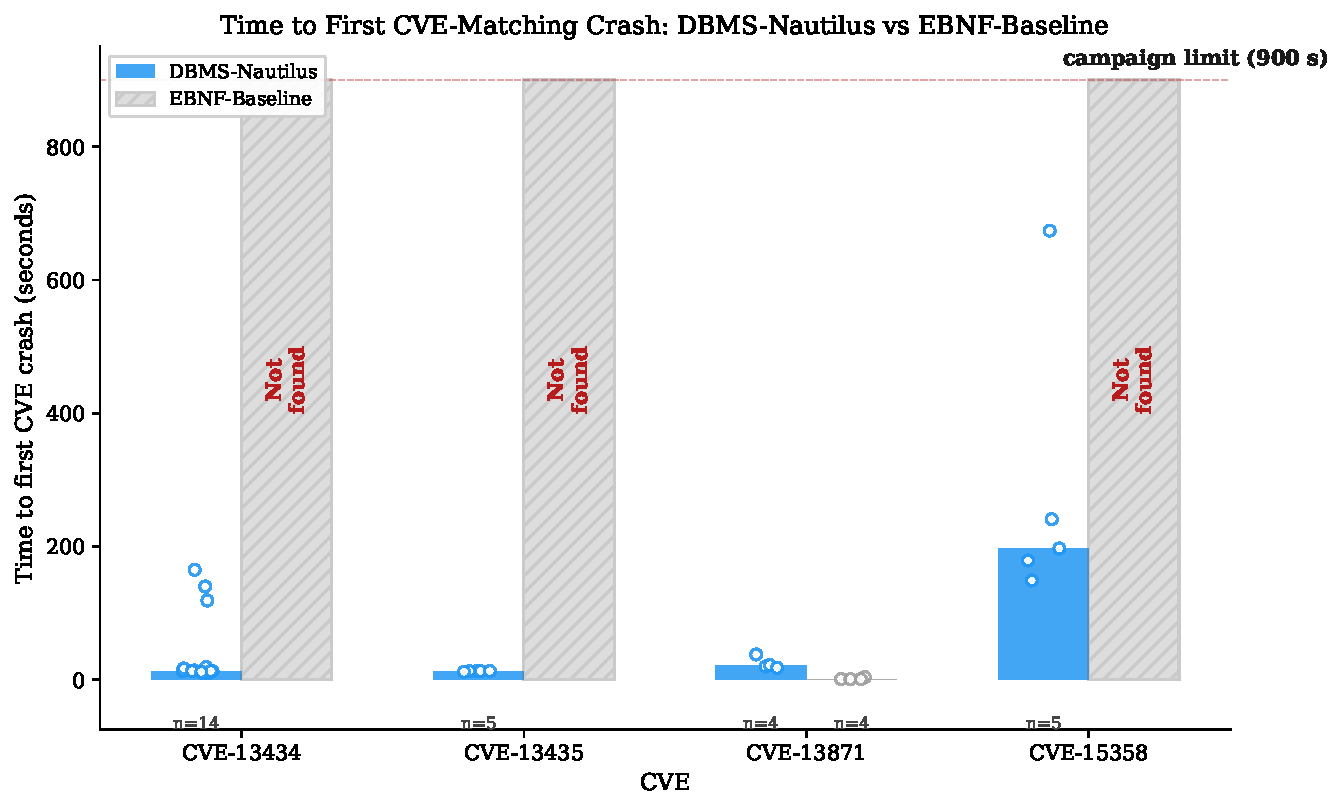
\includegraphics[width=\textwidth]{figures/fig_4_1_time_to_first_cve.pdf}
\caption{Time to first CVE-matching crash: DBMS-Nautilus vs EBNF-Baseline.}
\label{fig:time-to-cve}
\end{figure}

These results indicate that DBMS-Nautilus with seed rules achieves reliable CVE rediscovery for 4 of 4 target CVEs, with the majority of discoveries occurring within the first minutes of campaign execution.

\vspace{0.5em}
\noindent\fbox{\parbox{\dimexpr\linewidth-2\fboxsep-2\fboxrule}{%
\textbf{Answer to RQ1:} DBMS-Nautilus with seed rules reliably rediscovers 4 of 4 target CVEs (28/30 runs), with median time to first CVE crash ranging from 13\,s (CVE-2020-13435) to 197\,s (CVE-2020-15358). The EBNF-Baseline found only 1 of 4 CVEs (CVE-2020-13871), confirming that 3 of the 4 target vulnerabilities require domain-specific structural patterns that generic grammar specifications cannot express.}}
\vspace{0.5em}


\subsection{RQ2: Bug Detection}
\label{sec:rq2-results}

DBMS-Nautilus without seed rules discovers 13 distinct bug classes across 20 campaigns on 4 SQLite versions, producing 48 unique stack hashes after cross-campaign deduplication (individual campaigns produce many more hashes due to repeated discoveries; see RQ3 for per-campaign counts). The EBNF-Baseline discovers only 4 of the same 13 classes. Table~\ref{tab:rq2-comparison} compares the two grammars: for each bug class, it lists the versions on which each grammar triggered the bug and the number of unique stack hashes observed.

\begin{table}[htbp]
\caption{Bug classes discovered by each grammar.}
\label{tab:rq2-comparison}
\centering
\footnotesize
\setlength{\tabcolsep}{6pt}
\begin{tabular}{l >{\raggedright\arraybackslash}p{4.4cm} >{\raggedright\arraybackslash}p{2.5cm} >{\raggedright\arraybackslash}p{2.5cm} c}
\toprule
\textbf{Class} & \textbf{Bug Type} & \textbf{DBMS-Nautilus} & \textbf{EBNF-Baseline} & \textbf{Hashes} \\
\midrule
BC001 & Null ptr in \texttt{sqlite3\-Expr\-Code\-Target} & 3.30.1, 3.31.1, 3.32.0 & --- & 3 \\[1pt]
BC002 & Null ptr in \texttt{sqlite3\-Fts5\-Get\-Tokenizer} & 3.30.1, 3.31.1, 3.32.0, 3.32.2 & 3.30.1, 3.31.1, 3.32.0, 3.32.2 & 4/4 \\[1pt]
BC003 & Int overflow in \texttt{sqlite3\_str\_vappendf} & 3.30.1, 3.31.1, 3.32.0 & --- & 6 \\[1pt]
BC004 & Use-after-free in \texttt{Window\-Unlink\-From\-Select} & 3.30.1 & 3.30.1 & 1/1 \\[1pt]
BC005 & Float cast overflow in \texttt{alsoAnInt} & 3.31.1, 3.32.0, 3.32.2 & 3.30.1, 3.32.0 & 10/7 \\[1pt]
BC006 & Null ptr in \texttt{is\-Auxiliary\-Vtab\-Operator} & 3.31.1 & --- & 1 \\[1pt]
BC007 & Use-after-free in \texttt{reset\-Accumulator} & 3.30.1 & --- & 1 \\[1pt]
BC008 & Use-after-free in \texttt{sqlite3\-Expr\-Code\-Target} & 3.31.1 & --- & 13 \\[1pt]
BC009 & Float cast overflow in \texttt{Vdbe\-Mem\-Numerify} & 3.32.2 & --- & 2 \\[1pt]
BC010 & Null ptr in \texttt{sqlite3\-Select} & 3.31.1, 3.32.0 & --- & 2 \\[1pt]
BC011 & Heap use-after-free in \texttt{sqlite3\-Window\-List\-Delete} & 3.30.1 & 3.30.1 & 2/2 \\[1pt]
BC012 & Null ptr in \texttt{sqlite3\-Atoi64} & 3.30.1 & --- & 2 \\[1pt]
BC013 & Segfault in \texttt{sqlite3\-Expr\-Code\-Target} & 3.30.1 & --- & 1 \\
\midrule
\multicolumn{4}{l}{\textbf{Total: 13 classes (DBMS-Nautilus) vs 4 classes (EBNF-Baseline)}} & \textbf{48/14} \\
\bottomrule
\end{tabular}
\end{table}

The EBNF-Baseline's 4 classes (BC002, BC004, BC005, BC011) involve standard SQL constructs --- FTS virtual tables, window functions, and type casts --- that any comprehensive grammar exercises. The remaining 9 classes require domain-specific structural patterns absent from the EBNF grammar.

\begin{table}[htbp]
\caption{Bug classes per campaign by version.}
\label{tab:rq2-per-run}
\centering
\begin{tabular}{lcccc}
\toprule
\textbf{Grammar} & \textbf{3.30.1} & \textbf{3.31.1} & \textbf{3.32.0} & \textbf{3.32.2} \\
\midrule
\textbf{DBMS-Nautilus} & $\mathbf{7.0 \pm 1.0}$ & $\mathbf{6.0 \pm 0.7}$ & $\mathbf{4.4 \pm 0.5}$ & $\mathbf{2.4 \pm 0.9}$ \\
EBNF-Baseline & $2.8 \pm 0.8$ & $1.0 \pm 0.0$ & $1.2 \pm 0.5$ & $1.0 \pm 0.0$ \\
\midrule
\textbf{Ratio} & $2.5\times$ & $6.0\times$ & $3.7\times$ & $2.4\times$ \\
\bottomrule
\end{tabular}
\end{table}

Table~\ref{tab:rq2-per-run} breaks down the per-campaign discovery rate by version. DBMS-Nautilus finds $7.0 \pm 1.0$ bug classes per campaign on version~3.30.1 ($2.5\times$ more than the EBNF-Baseline's $2.8 \pm 0.8$), rising to $6.0\times$ on version~3.31.1 where the EBNF-Baseline finds only $1.0$ class per campaign. The advantage is smallest on version~3.32.2 ($2.4\times$), where fewer bugs remain after upstream fixes.

Four of the 13 bug classes match known CVEs by crash-line verification against the official proof-of-concept inputs: BC001 (CVE-2020-13435), BC003 (CVE-2020-13434), BC006 (CVE-2020-9327), and BC007 (CVE-2020-13871). These rediscoveries occurred without dedicated seed rules, confirming that the grammar's structural primitives can compositionally reconstruct CVE-triggering inputs. The remaining 9 classes have no CVE assignment; cross-version replay against 19 SQLite versions (3.26.0 through 3.53.0) on production (non-sanitizer) builds shows that 6 of them (BC004, BC008, BC010, BC011, BC012, BC013) cause segmentation faults across up to 10 consecutive releases.

\needspace{20\baselineskip}
\subsubsection{Selected Bugs}

Five representative bugs illustrate the kinds of defects that the grammar's structural compositions expose. The full list of 13 bug classes is summarized in Table~\ref{tab:rq2-comparison}.

\textbf{Null pointer in SELECT processing exposed by recursive CTE (BC010).} A recursive CTE combined with an \texttt{EXCEPT} operator and a window \texttt{FILTER} clause causes the query compiler to dereference a null \texttt{Table} pointer inside \texttt{sqlite3Select} (Listing~\ref{lst:bc010}). The grammar's \texttt{Recursive-CTE} and \texttt{Window-Func} non-terminals jointly produce this combination; neither construct appears in isolation in the EBNF-Baseline. The bug causes segmentation faults on production builds across six consecutive releases (3.30.0--3.32.2); no CVE was assigned. The EBNF-Baseline never triggered this path.

\begin{lstlisting}[caption={BC010: Null pointer in \texttt{sqlite3Select}.},label={lst:bc010},language=SQL,numbers=none]
-- Trigger SQL
WITH RECURSIVE a(x) AS (
  SELECT 1 UNION ALL SELECT x+1 FROM a WHERE x < 5
), b(y) AS (
  SELECT TRUE IN (VALUES (NULL)
    EXCEPT SELECT CURRENT_TIMESTAMP
    ORDER BY CURRENT_TIMESTAMP COLLATE NOCASE)
  FROM a
)
SELECT *, count(*) FILTER (WHERE RAISE(IGNORE))
  OVER (PARTITION BY RAISE(IGNORE)
        ORDER BY CURRENT_TIME DESC NULLS LAST
        ROWS BETWEEN CURRENT ROW AND UNBOUNDED FOLLOWING)
FROM b;

-- UBSan diagnostic
-- runtime error: member access within null pointer
--   of type 'Table' (aka 'struct Table')
-- in sqlite3Select
\end{lstlisting}

\textbf{Use-after-free with sanitizer blind spot (BC008).} A self-join with a correlated subquery combining \texttt{lead()} and \texttt{SUM()} triggers a misaligned memory access in the expression code generator (Listing~\ref{lst:bc008}). The misaligned address (\texttt{0x1ffffcaaaf0b}) confirms access to freed memory fill-pattern bytes. This bug exhibits a sanitizer blind spot on version~3.32.0: the ASan+UBSan build reports no error while the production build segfaults --- \texttt{SQLITE\_DEBUG} assertions mask the defect in instrumented builds. Affects 9 versions (3.26.0--3.32.0); fixed in 3.32.1. The 13 unique stack hashes reflect a rich space of triggering paths. The EBNF-Baseline cannot generate this self-join pattern.

\begin{lstlisting}[caption={BC008: Use-after-free in \texttt{sqlite3ExprCodeTarget}.},label={lst:bc008},language=SQL,numbers=none]
-- Trigger SQL
CREATE TABLE p(a UNIQUE);
SELECT p.a FROM p JOIN p q ON 3 = p.a
  NATURAL JOIN p
  WHERE p.a IN((
    SELECT(SELECT coalesce(lead(2) OVER(), SUM(a)))
    FROM p d WHERE p.a
  ));

-- UBSan diagnostic (3.31.1)
-- runtime error: member access within misaligned address
--   0x1ffffcaaaf0b for type 'struct AggInfo_func'
-- Stack: sqlite3ExprCodeTarget -> sqlite3ExprCodeExprList
--        -> innerLoopLoadRow -> selectInnerLoop
\end{lstlisting}

\textbf{Heap use-after-free in window list cleanup (BC011).} ASan confirms a heap-use-after-free in \texttt{sqlite3WindowListDelete} when a \texttt{Select} node whose window list was already deallocated is freed a second time (Listing~\ref{lst:bc011}). The trigger requires a \texttt{CHECK} constraint enclosing a window function inside a compound query --- a combination produced by the grammar's \texttt{Stress-Query} and \texttt{Validation-Op} non-terminals. Affects 3.26.0--3.30.1; fixed in 3.31.1. Both grammars found this bug, confirming that window functions are reachable through generic SQL.

\begin{lstlisting}[caption={BC011: Heap use-after-free in \texttt{sqlite3WindowListDelete}.},label={lst:bc011},language=SQL,numbers=none]
-- Trigger SQL
CREATE TABLE t3 (c1 TEXT CHECK ((SELECT * LIMIT EXISTS
  (SELECT * INTERSECT SELECT * FROM t1 WHERE CURRENT_DATE
   GROUP BY FALSE WINDOW w1 AS ()
   ORDER BY CURRENT_TIMESTAMP COLLATE NOCASE ASC),
  RAISE(IGNORE)))) WITHOUT ROWID;

-- ASan diagnostic
-- ERROR: AddressSanitizer: heap-use-after-free
-- READ of size 8 at 0xf531e6c029b8 thread T0
-- #0 sqlite3WindowListDelete -> clearSelect
--    -> sqlite3SelectDelete -> sqlite3ExprDeleteNN
\end{lstlisting}

\textbf{CVE-2020-9327 rediscovery via generated column composition (BC006).} The query planner dereferences a null \texttt{Table} pointer when classifying operators for a view that references a generated column with a \texttt{UNIQUE} constraint (Listing~\ref{lst:bc006}). Rediscovering this CVE requires four structural elements from different grammar groups --- \texttt{GENERATED ALWAYS AS}, \texttt{UNIQUE}, \texttt{CREATE VIEW}, and a multi-table join --- produced jointly by the grammar's \texttt{Schema-Setup} and \texttt{Stress-Query} non-terminals. Affects 3.31.1 only; fixed in 3.32.0. The EBNF-Baseline has no generated column rules and cannot reach this path.

\begin{lstlisting}[caption={BC006: Null pointer in \texttt{isAuxiliaryVtabOperator} (CVE-2020-9327).},label={lst:bc006},language=SQL,numbers=none]
-- Trigger SQL
CREATE TABLE v0(v3, v1 GENERATED ALWAYS AS (v3) UNIQUE);
CREATE TABLE v5(v6 UNIQUE, v7 UNIQUE);
CREATE VIEW v8 AS
  SELECT coalesce(v3, v1) AS v9 FROM v0 WHERE v1 IN('');
SELECT * FROM v8 JOIN v5 WHERE 0 > v7 AND v9 OR v6 = ' ';

-- UBSan diagnostic
-- runtime error: member access within null pointer
--   of type 'Table' (aka 'struct Table')
-- Stack: isAuxiliaryVtabOperator -> exprAnalyze
--        -> sqlite3WhereExprAnalyze -> sqlite3WhereBegin
\end{lstlisting}

\textbf{Use-after-free in window function unlinking (BC004).} A view definition combined with an \texttt{ORDER BY} clause inside a compound query triggers a store to a misaligned address during window function cleanup (Listing~\ref{lst:bc004}). The address \texttt{0xaaaaaaaaaaaaaaaa} is the \texttt{SQLITE\_DEBUG} freed-memory fill pattern, confirming that the code writes through a dangling pointer. The resulting segfault is non-deterministic on production builds. Affects 3.30.0--3.30.1; fixed in 3.31.1. Both grammars found this bug, indicating that view-plus-window combinations are exercised even by generic SQL generation.

\begin{lstlisting}[caption={BC004: Use-after-free in \texttt{sqlite3WindowUnlinkFromSelect}.},label={lst:bc004},language=SQL,numbers=none]
-- Trigger SQL
CREATE TABLE IF NOT EXISTS p(a INTEGER);
CREATE TABLE IF NOT EXISTS q(b INTEGER);
CREATE VIEW IF NOT EXISTS vp AS SELECT a FROM p ORDER BY a;
SELECT (SELECT t2.* FROM r NOT INDEXED WHERE FALSE COLLATE
  RTRIM UNION SELECT FALSE FROM t1 WHERE CURRENT_TIME
  COLLATE RTRIM GROUP BY TRUE NOT NULL HAVING NULL
  WINDOW w1 AS (PARTITION BY CURRENT_TIME)
  ORDER BY quote(CURRENT_DATE COLLATE RTRIM GLOB FALSE
  COLLATE NOCASE >= TRUE) DESC NULLS LAST)
  AS z39y_3sry46f___gb75,
  FALSE COLLATE BINARY AS gu571__i14_6_d_3f1_9__o
FROM p, q
WHERE p.a = (SELECT 0 INTERSECT SELECT b FROM vp)
  AND p.a = 0;

-- UBSan diagnostic
-- runtime error: store to misaligned address
--   0xaaaaaaaaaaaaaaaa for type 'Window *'
--   (requires 8 byte alignment) -- freed memory pattern
-- in sqlite3WindowUnlinkFromSelect
\end{lstlisting}

\vspace{0.5em}
\noindent\fbox{\parbox{\dimexpr\linewidth-2\fboxsep-2\fboxrule}{%
\textbf{Answer to RQ2:} DBMS-Nautilus discovers 13 bug classes (48 hashes) without seed rules, including 4 CVE rediscoveries and 6 non-CVE bugs that cause segmentation faults on production builds across up to 10 consecutive releases. The EBNF-Baseline finds 4 of the 13 classes (14 hashes); 9 bug classes are exclusive to DBMS-Nautilus.}}
\vspace{0.5em}


\subsection{RQ3: Performance Trade-off}
\label{sec:rq3-results}

DBMS-Nautilus and the EBNF-Baseline were compared across four metrics using the Mann-Whitney~$U$ test with Cliff's~$d$ effect size (Table~\ref{tab:rq3-stats}). Each cell reports mean $\pm$ standard deviation; $n=5$ per cell except EBNF-Baseline 3.32.0 where $n=4$.

\begin{table}[htbp]
\caption{Statistical comparison: DBMS-Nautilus vs EBNF-Baseline.}
\label{tab:rq3-stats}
\centering
\resizebox{\textwidth}{!}{%
\begin{tabular}{llrrrl}
\toprule
\textbf{Metric} & \textbf{Version} & \textbf{DBMS-Nautilus} & \textbf{EBNF-Baseline} & \textbf{$p$-value} & \textbf{Cliff's $d$} \\
\midrule
\multirow{4}{*}{Unique RCs}
  & 3.30.1 & $\mathbf{215.4 \pm 24.4}$ & $3.6 \pm 2.1$ & 0.012 & $+1.00$ (large) \\
  & 3.31.1 & $\mathbf{170.6 \pm 72.4}$ & $1.0 \pm 0.0$ & 0.007 & $+1.00$ (large) \\
  & 3.32.0 & $\mathbf{139.4 \pm 73.0}$ & $2.0 \pm 2.0$ & 0.018 & $+1.00$ (large) \\
  & 3.32.2 & $\mathbf{296.8 \pm 38.2}$ & $1.0 \pm 0.0$ & 0.007 & $+1.00$ (large) \\
\midrule
\multirow{4}{*}{Edge Cov.}
  & 3.30.1 & $19{,}862 \pm 274$ & $\mathbf{23{,}323 \pm 152}$ & 0.008 & $-1.00$ (large) \\
  & 3.31.1 & $20{,}010 \pm 915$ & $\mathbf{23{,}182 \pm 341}$ & 0.008 & $-1.00$ (large) \\
  & 3.32.0 & $20{,}017 \pm 1{,}109$ & $\mathbf{23{,}645 \pm 300}$ & 0.016 & $-1.00$ (large) \\
  & 3.32.2 & $20{,}838 \pm 177$ & $\mathbf{23{,}811 \pm 166}$ & 0.008 & $-1.00$ (large) \\
\midrule
\multirow{4}{*}{Throughput}
  & 3.30.1 & $90.7 \pm 7.1$ & $\mathbf{196.3 \pm 15.9}$ & 0.008 & $-1.00$ (large) \\
  & 3.31.1 & $92.6 \pm 14.1$ & $\mathbf{182.7 \pm 12.2}$ & 0.008 & $-1.00$ (large) \\
  & 3.32.0 & $84.9 \pm 10.8$ & $\mathbf{198.0 \pm 11.8}$ & 0.016 & $-1.00$ (large) \\
  & 3.32.2 & $95.2 \pm 9.3$ & $\mathbf{182.4 \pm 15.8}$ & 0.008 & $-1.00$ (large) \\
\midrule
\multirow{4}{*}{TTFC (s)}
  & 3.30.1 & $1.8 \pm 0.8$ & $1.8 \pm 1.3$ & 0.821 & $+0.12$ (negl.) \\
  & 3.31.1 & $1.8 \pm 0.4$ & $\mathbf{1.2 \pm 0.4}$ & 0.093 & $+0.60$ (large) \\
  & 3.32.0 & $1.6 \pm 0.9$ & $\mathbf{1.0 \pm 0.0}$ & 0.240 & $+0.40$ (medium) \\
  & 3.32.2 & $2.0 \pm 0.7$ & $\mathbf{1.8 \pm 1.1}$ & 0.740 & $+0.16$ (small) \\
\bottomrule
\end{tabular}}
\end{table}

The results reveal a clear trade-off between structural complexity and raw throughput. The EBNF-Baseline achieves $1.9\times$--$2.3\times$ higher throughput (mean 189.9 executions per second vs 90.8 for DBMS-Nautilus) and $1.1\times$--$1.2\times$ higher edge coverage (mean 23{,}490 vs 20{,}182 edges). However, DBMS-Nautilus discovers $60\times$--$297\times$ more unique root causes per campaign (mean 205.6 vs 1.9), with large effect sizes ($d = 1.00$, $p < 0.05$) on all four versions.

Time to first crash (TTFC) shows no statistically significant difference between the two grammars on any version ($p > 0.05$ on all four), indicating that both grammars find their first crash within seconds of campaign start. The throughput disadvantage of DBMS-Nautilus does not translate into a delay in initial crash discovery.

Figure~\ref{fig:coverage-growth} shows the edge coverage growth over the 15-minute campaign duration for both grammars. The EBNF-Baseline reaches higher absolute coverage due to its higher throughput and broader syntactic variety, but DBMS-Nautilus's coverage growth rate suggests that it explores a smaller but more crash-producing subset of the code.

\begin{figure}[htbp]
\centering
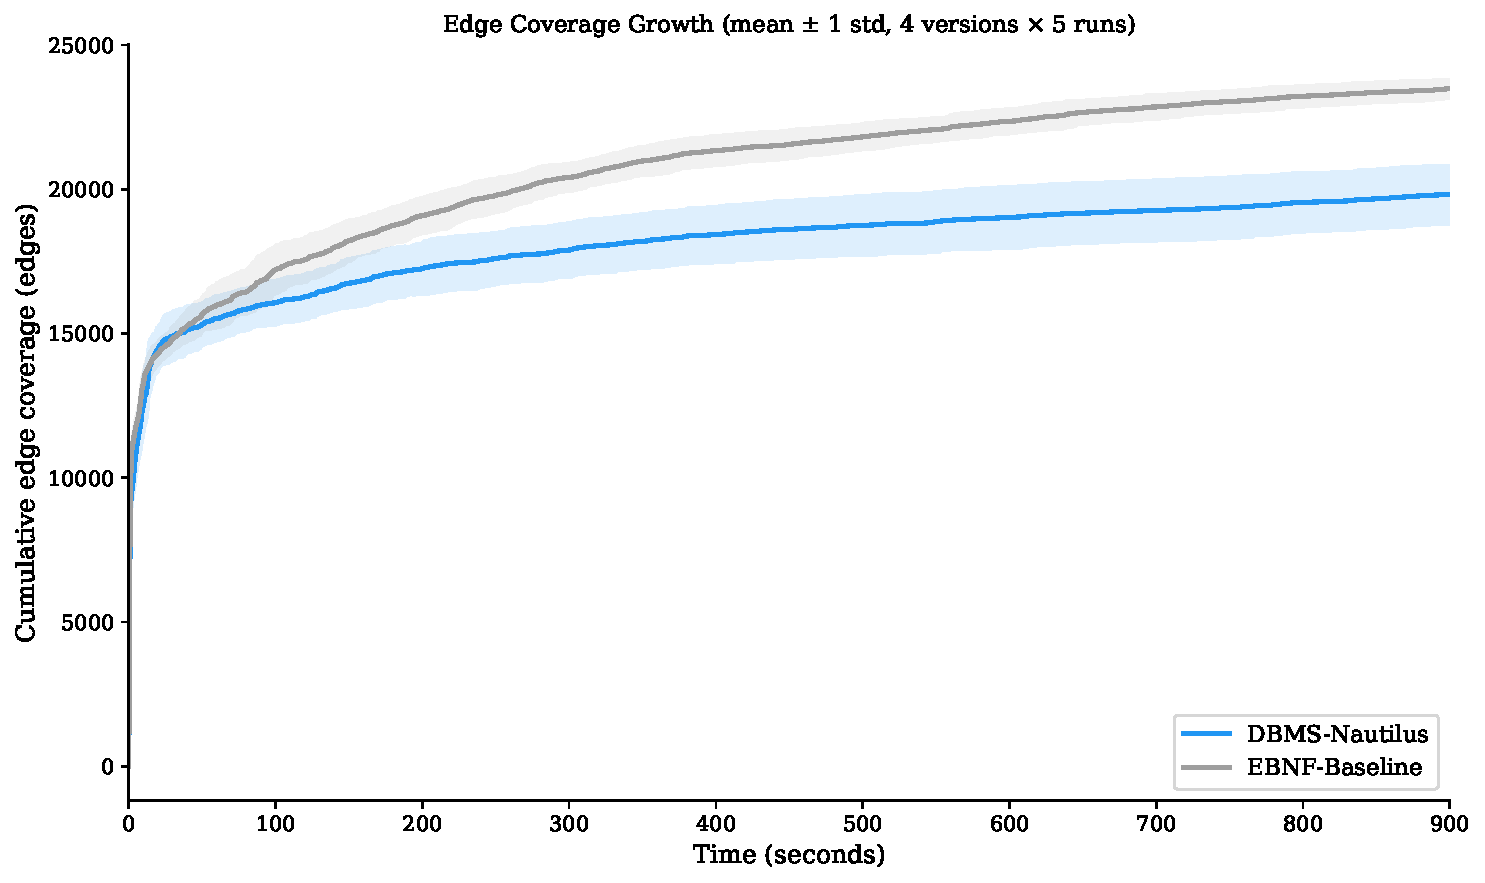
\includegraphics[width=\textwidth]{figures/fig_4_3_coverage_growth.pdf}
\caption{Edge coverage growth over time.}
\label{fig:coverage-growth}
\end{figure}

The EBNF-Baseline's simpler production rules generate shorter SQL inputs, yielding faster execution per test case; Figure~\ref{fig:throughput} shows throughput across all four versions.

\begin{figure}[htbp]
\centering
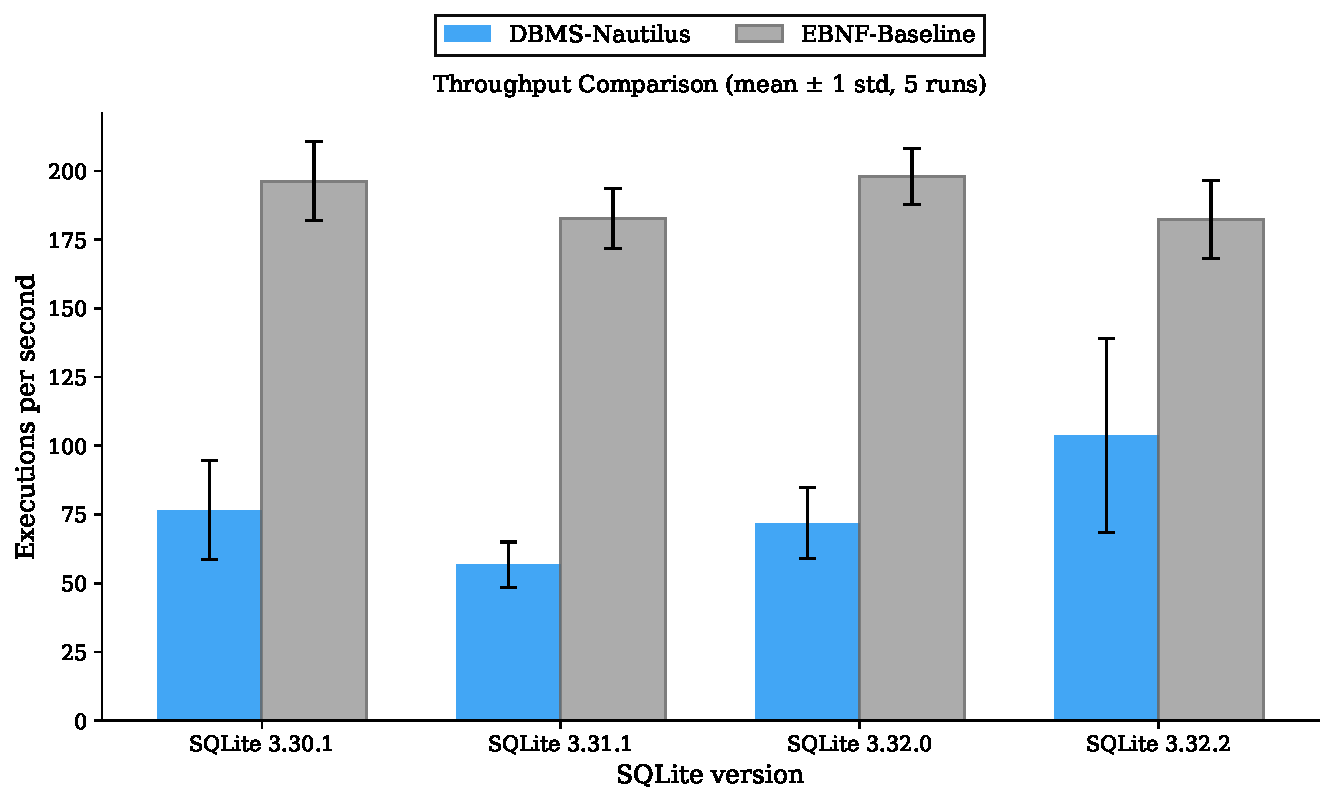
\includegraphics[width=\textwidth]{figures/fig_4_4_throughput.pdf}
\caption{Throughput comparison across SQLite versions.}
\label{fig:throughput}
\end{figure}

Figure~\ref{fig:ttfc} shows the time-to-first-crash distribution; both grammars find their first crash within seconds on every version, confirming that the throughput gap does not delay initial crash discovery.

\begin{figure}[htbp]
\centering
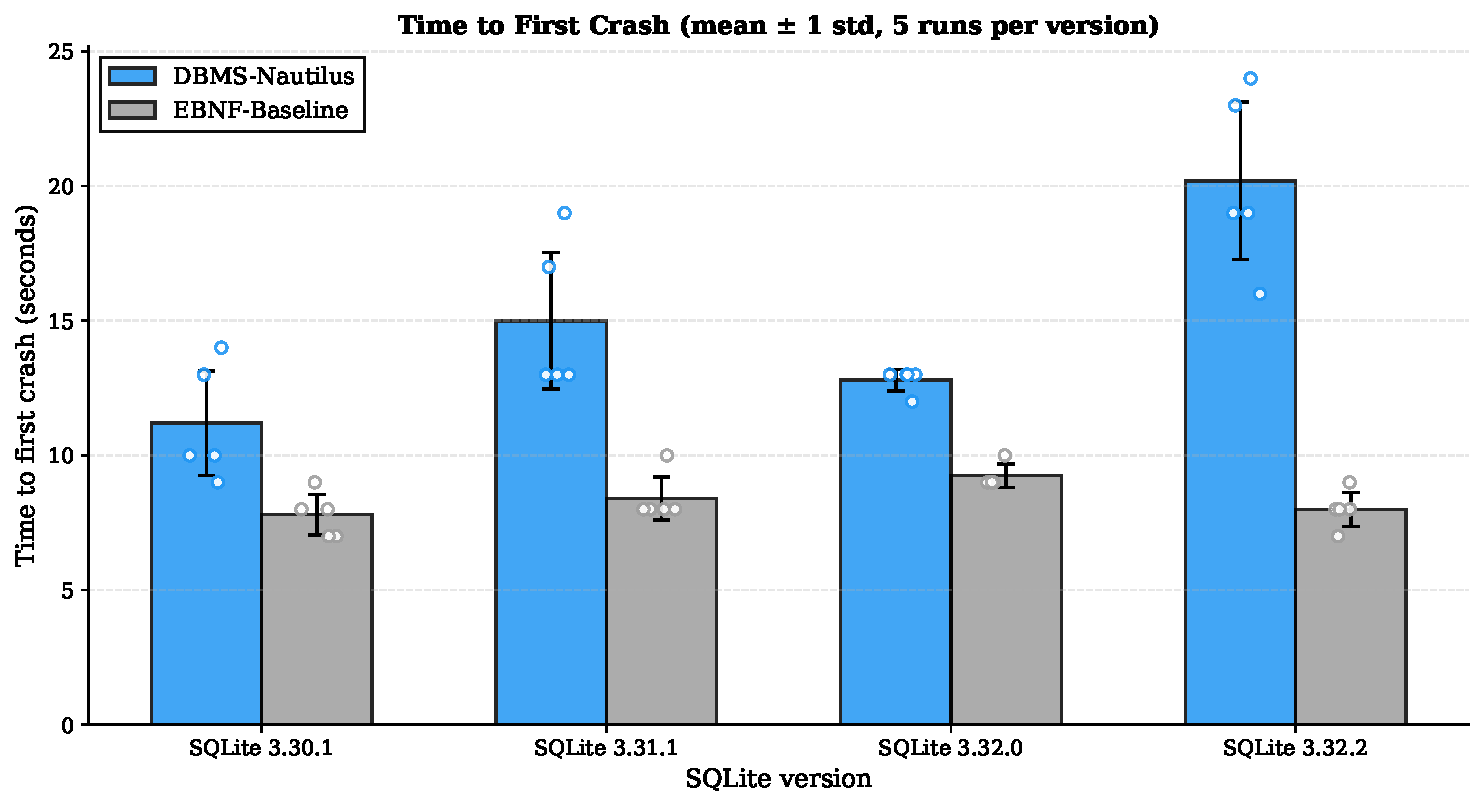
\includegraphics[width=\textwidth]{figures/fig_4_5_time_to_first_crash.pdf}
\caption{Time to first UBSan/ASan crash (excluding debug assertions).}
\label{fig:ttfc}
\end{figure}

DBMS-Nautilus sacrifices throughput and edge coverage breadth in exchange for higher crash diversity: structural complexity in grammar design redirects fuzzing effort toward code paths that produce crashes, at the cost of raw execution speed.

\vspace{0.5em}
\noindent\fbox{\parbox{\dimexpr\linewidth-2\fboxsep-2\fboxrule}{%
\textbf{Answer to RQ3:} DBMS-Nautilus discovers $108\times$ more unique root causes per campaign (205.6 vs 1.9) at the cost of 52.1\% lower throughput and 14.1\% lower edge coverage. The throughput reduction does not delay initial crash discovery: time to first crash shows no statistically significant difference between the two grammars ($p > 0.05$ on all versions). The EBNF-Baseline's higher coverage is shallow --- it executes more inputs but the additional coverage does not translate into proportional crash discovery.}}
\vspace{0.5em}


\section{Discussion}
\label{sec:discussion}

\subsection{Qualitative Analysis}
\label{sec:qualitative}

The 13 bug classes discovered by DBMS-Nautilus (RQ2) were validated through cross-version testing against 19 SQLite releases (3.26.0 through 3.53.0) using both sanitizer-instrumented and production (no-sanitizer) harness builds.

\emph{CVE-matching bugs} (4 classes, 30.8\% of total). BC001 (CVE-2020-13435), BC003 (CVE-2020-13434), BC006 (CVE-2020-9327), and BC007 (CVE-2020-13871) are rediscoveries of known CVEs through compositional generation without seed rules. These validate the grammar's primary design objective: encoding crash-producing patterns that can reconstruct CVE-triggering inputs without embedding proof-of-concept strings. For BC001, the grammar's join and window function patterns trigger a null pointer dereference in the expression code generator, matching CVE-2020-13435. For BC003, the \texttt{Boundary-Func-Call} non-terminal produces a \texttt{printf} call with \texttt{INT\_MAX} precision, matching CVE-2020-13434. For BC006, the combination of generated column, \texttt{UNIQUE} constraint, view, and join matches CVE-2020-9327. For BC007, the combination of window function, aggregate, and \texttt{EXCEPT} compound operator triggers a use-after-free in \texttt{resetAccumulator}, matching CVE-2020-13871.

\emph{Non-CVE production bugs} (6 classes, 46.2\% of total). BC004, BC008, BC010, BC011, BC012, and BC013 cause segmentation faults on production builds and were fixed between versions 3.31.1 and 3.32.3 without CVE assignment. BC008 and BC013 each affect 9--10 consecutive SQLite versions. BC010 affects 6 versions (3.30.0--3.32.2). BC008 exhibits a sanitizer blind spot on version~3.32.0: the ASan+UBSan build reports no error while the production build segfaults.

\emph{Sanitizer-only bugs} (3 classes, 23.1\% of total). BC002, BC005, and BC009 trigger UBSan diagnostics but do not crash production builds on x86\_64. BC002 (FTS5 tokenizer null pointer) persists across 15 versions until 3.36.0.

\subsection{Failure Cases and Limitations}
\label{sec:limitations}

At least two concrete limitations of the proposed approach were identified during the evaluation:

\begin{enumerate}
  \item \textbf{Context-free grammar cannot enforce semantic validity.} The grammar is context-free and cannot enforce type correctness, referential integrity, or valid column count matching between \texttt{INSERT} values and table definitions. Semantically invalid SQL statements are generated and immediately rejected by SQLite's parser or query planner, consuming execution time without contributing to coverage. The throughput gap between DBMS-Nautilus (90.8 execs/sec) and the EBNF-Baseline (189.9 execs/sec) is partially attributable to DBMS-Nautilus generating longer, more complex inputs that take more time to parse and reject.

  \item \textbf{Manual CVE analysis dependency.} The DBMS-Nautilus methodology requires manual expertise to identify which SQL constructs are relevant to each vulnerability. The effectiveness of the approach depends on the quality of this analysis: if a critical structural pattern is missed or incorrectly characterized, the corresponding grammar rules will be absent or ineffective. Automating this analysis --- for example, through differential code analysis between patched and unpatched versions --- is an open research question.
\end{enumerate}

\subsection{Threats to Validity}
\label{sec:threats}

\paragraph{Internal validity.}
Stack-hash deduplication using the top 5 frames is a heuristic that may both over-count and under-count bug classes. Over-counting occurs when two manifestations of the same root cause crash through different call paths; under-counting occurs when distinct bugs crash through the same 5-frame sequence. The \texttt{SQLITE\_DEBUG} build flag introduces an additional confound: it fills freed memory with \texttt{0xAA} bytes, causing use-after-free bugs to manifest as misaligned-access diagnostics rather than heap-use-after-free reports. This was addressed through no-debug harness replay for CVE confirmation (see Table~\ref{tab:cve-rediscovery}), but may affect the classification accuracy of non-CVE bug classes. Campaign durations of 15~minutes may miss bugs requiring longer exploration or rarer compositional combinations; however, extending campaigns introduces diminishing returns in coverage-guided fuzzing.

\paragraph{External validity.}
All experiments target a single DBMS --- SQLite~\citep{sqlite} --- with a single input language (SQL). SQLite is an embedded database with a compact codebase (${\sim}$150{,}000 lines of C), and its bug landscape may not be representative of larger server-based systems such as MySQL or PostgreSQL. The comparison uses a single baseline grammar (EBNF-Baseline) rather than multiple baselines or existing fuzzing tools such as SQLsmith~\citep{sqlsmith} or Squirrel~\citep{squirrel}. Direct comparison with these tools was not feasible because they use fundamentally different fuzzing strategies (query-plan-guided generation for SQLsmith, AST-level mutation for Squirrel) that cannot be isolated to a grammar-only comparison. The EBNF-Baseline isolates the effect of grammar design by holding all other variables constant.

\paragraph{Construct validity.}
The 80\% fidelity threshold for CVE signature matching is an arbitrary cutoff. A higher threshold would reduce false positive matches but might miss legitimate rediscoveries where the stack trace differs due to compiler optimizations or ASan instrumentation overhead. The sanitizer oracle misses entire categories of bugs: logic bugs producing incorrect results without undefined behavior, and denial-of-service bugs causing non-termination without crashing. Edge coverage as measured by the AFL-style bitmap is subject to hash collisions, where distinct edges map to the same bitmap byte, potentially causing the fuzzer to miss coverage-increasing inputs.

\subsection{Summary}
\label{sec:summary}

The experimental evaluation demonstrates three principal findings. First, DBMS-Nautilus with seed rules reliably rediscovers 4 out of 4 target CVEs across 20 campaigns, supporting the hypothesis that domain-knowledge-driven grammar engineering can reconstruct CVE-triggering inputs from independently encoded structural primitives (RQ1). Second, DBMS-Nautilus without seed rules discovers 13 distinct bug classes (48 unique hashes), validated through cross-version testing against 19 SQLite releases: 4 are CVE rediscoveries, 6 are non-CVE production bugs affecting up to 10 consecutive releases each, and 3 are sanitizer-only detections (RQ2). Nine of the 13 bug classes were found exclusively by DBMS-Nautilus. Third, DBMS-Nautilus sacrifices throughput ($2.1\times$ slower) and edge coverage (14.1\% lower) in exchange for $108\times$ more unique root causes per campaign, indicating that structural complexity redirects fuzzing effort toward crash-producing code at the cost of raw execution speed (RQ3). The EBNF-Baseline found 4 of the 13 bug classes (BC002, BC004, BC005, BC011), none of which match the 4 CVE-rediscovery classes.
\newpage\cleardoublepage
\chapter*{Conclusion}
\addcontentsline{toc}{chapter}{Conclusion}

This thesis presented DBMS-Nautilus, a grammar-based greybox fuzzing system for automated vulnerability detection in SQLite. What makes DBMS-Nautilus different is its grammar: the grammar determines what the fuzzer can discover, while the fuzzing engine navigates within that space but cannot expand it. The central contribution is a grammar engineering methodology based on structural primitives --- SQL patterns extracted from CVE root-cause analysis, encoded as composable production rules without hardcoding any proof-of-concept inputs. The cross-pollination property of this design, where a single non-terminal serves multiple CVEs simultaneously and the fuzzer freely composes patterns across independent non-terminal groups, enables compositional discovery of vulnerability-triggering inputs.

The grammar contains 526 production rules, iteratively refined based on experimental evidence.

Regarding the first research question, DBMS-Nautilus successfully rediscovered all four target CVEs through compositional grammar generation: CVE-2020-13434 (integer overflow in printf, 14/15 version-runs), CVE-2020-13435 (null pointer dereference, 5/5 runs), CVE-2020-13871 (use-after-free in window function processing, 4/5 runs), and CVE-2020-15358 (heap buffer overflow, 5/5 runs). None of these were found by embedding proof-of-concept inputs --- the fuzzer independently composed the triggering SQL from separate structural primitives. The EBNF-Baseline found only 1 of 4 CVEs (CVE-2020-13871), confirming that 3 of the 4 target vulnerabilities require domain-specific structural patterns.

Regarding the second research question, DBMS-Nautilus discovered 13 distinct bug classes across 48 unique stack hashes spanning four SQLite versions: 4 are CVE rediscoveries without dedicated seed rules (BC001=CVE-2020-13435, BC003=CVE-2020-13434, BC006=CVE-2020-9327, BC007=CVE-2020-13871), 6 are non-CVE bugs that cause crashes on production builds across up to 10 consecutive releases, and 3 are sanitizer-only detections. Nine of the 13 bug classes were found exclusively by DBMS-Nautilus. The discovery of bugs beyond the grammar's explicit design targets confirms the cross-pollination hypothesis: structural patterns intended for specific CVEs also exercise adjacent code paths containing previously undocumented defects.

Regarding the third research question, the proposed grammar sacrifices throughput ($2.1\times$ slower) and edge coverage (14.1\% lower) in exchange for $108\times$ more unique root causes per campaign compared to a generic EBNF baseline grammar, with large effect sizes ($d = 1.00$, $p < 0.05$) on all four versions. This asymmetry is consistent with the hypothesis that structural complexity concentrates fuzzing effort on vulnerability-relevant code paths at the cost of raw execution speed.

Several limitations bound these findings. All experiments target a single DBMS (SQLite), and the results may not generalize to larger server-based systems. The context-free grammar cannot enforce semantic constraints, meaning a fraction of generated inputs are rejected at runtime. The sanitizer-based oracle misses non-crash bugs such as infinite loops and incorrect query results. The grammar design process requires manual domain expertise in both SQL internals and vulnerability patterns.

Four directions warrant further investigation. First, reinforcement learning integration could enable adaptive weight tuning based on coverage and crash-frequency signals, potentially accelerating discovery of bugs requiring rare compositional combinations. Second, cross-DBMS grammar portability should be tested by adapting the structural primitives methodology to MySQL and PostgreSQL. Third, semantic-aware generation extending the grammar with type constraints would reduce wasted executions on semantically invalid inputs. Fourth, automated grammar expansion using large language model analysis of vulnerability disclosures could partially automate the grammar design process.
\newpage\cleardoublepage

\phantomsection
\addcontentsline{toc}{chapter}{References}
\bibliography{references}\newpage\cleardoublepage
\end{document}
